\documentclass[11pt,a4paper]{article}
\usepackage[a4paper,margin=25mm,headheight=15pt]{geometry}
\usepackage[T1]{fontenc}
\usepackage[utf8]{inputenc}
\usepackage{lmodern}
\usepackage{microtype}
\usepackage{setspace}
\usepackage{booktabs}
\usepackage{array}
\usepackage{tabularx}
\usepackage{longtable}
\usepackage{enumitem}
\usepackage{xcolor}
\usepackage{hyperref}
\usepackage{amsmath,amssymb,amsthm,mathtools}
\usepackage{graphicx}
\usepackage{tikz}
\usepackage{fancyhdr}
\usepackage{listings}
\usepackage{caption}
\usepackage{float}
\usepackage{url}
\usepackage{multirow}
\usepackage{ragged2e}
\usepackage[nameinlink,capitalize]{cleveref}
\usetikzlibrary{arrows.meta,positioning,fit,calc,shapes.geometric,backgrounds,matrix}

\definecolor{LinkBlue}{HTML}{1F4E79}
\definecolor{SoftBlue}{HTML}{EAF1F7}
\definecolor{SoftGray}{HTML}{F4F4F4}
\definecolor{MidGray}{HTML}{666666}
\definecolor{DarkText}{HTML}{1A1A1A}
\definecolor{Warn}{HTML}{8A4B08}
\definecolor{Safe}{HTML}{1B6B3A}
\definecolor{DeepRed}{HTML}{911926}

\hypersetup{
  colorlinks=true,
  linkcolor=LinkBlue,
  citecolor=LinkBlue,
  urlcolor=LinkBlue,
  pdftitle={AI Native Workflow 5.6.39: Long-Horizon Research, Human Attention, Hierarchical Execution, and Evidence Control},
  pdfauthor={Yuhe Sui}
}
\setlist[itemize]{topsep=4pt,itemsep=2pt,parsep=0pt,leftmargin=*}
\setlist[enumerate]{topsep=4pt,itemsep=3pt,parsep=0pt,leftmargin=*}
\renewcommand{\arraystretch}{1.16}
\setstretch{1.045}
\captionsetup{font=small,labelfont=bf}
\pagestyle{fancy}
\fancyhf{}
\fancyhead[L]{\small AI Native Workflow 5.6: Detailed Technical Report}
\fancyhead[R]{\small Version 5.6.39}
\fancyfoot[C]{\thepage}
\renewcommand{\headrulewidth}{0.3pt}
\renewcommand{\footrulewidth}{0pt}

\newcommand{\code}[1]{\texttt{\detokenize{#1}}}
\newcommand{\supported}{\textbf{Supported finding}}
\newcommand{\inference}{\textbf{Architectural inference}}
\newcommand{\hypothesis}{\textbf{Operational hypothesis}}
\newcommand{\observation}{\textbf{Practitioner observation}}
\newcommand{\unknown}{\textbf{Not publicly established}}
\newcolumntype{Y}{>{\RaggedRight\arraybackslash}X}
\newcolumntype{P}[1]{>{\RaggedRight\arraybackslash}p{#1}}
\newtheorem{definition}{Definition}[section]
\newtheorem{assumption}[definition]{Assumption}
\newtheorem{theorem}[definition]{Theorem}
\newtheorem{proposition}[definition]{Proposition}
\newtheorem{corollary}[definition]{Corollary}
\newtheorem{lemma}[definition]{Lemma}
\newtheorem{remark}[definition]{Remark}
\newcommand{\State}{\mathcal S}
\newcommand{\Trace}{\mathcal T}
\newcommand{\Evidence}{\mathcal E}
\newcommand{\Keys}{\mathcal K}
\newcommand{\Acc}{\operatorname{Acc}}
\newcommand{\llbracket}{[\![}
\newcommand{\rrbracket}{]\!]}
\newcommand{\Reach}{\operatorname{Reach}}
\newcommand{\Desc}{\operatorname{Desc}}
\newcommand{\proj}{\operatorname{proj}}

\lstdefinestyle{workflow}{
  basicstyle=\ttfamily\small,
  backgroundcolor=\color{SoftGray},
  frame=single,
  rulecolor=\color{black!20},
  breaklines=true,
  columns=fullflexible,
  keepspaces=true,
  showstringspaces=false,
  xleftmargin=4pt,
  xrightmargin=4pt,
  aboveskip=7pt,
  belowskip=7pt
}

\title{\vspace{-8mm}\textbf{AI Native Workflow 5.6}\\[2mm]
\large Detailed Rationale, Hierarchical Execution Architecture, Human-Attention-Aware Oversight, and Evidence Control}
\author{Yuhe Sui}
\date{3 September 2026\\Version 5.6.39}

\begin{document}
\maketitle

\begin{abstract}
Researchers increasingly compose frontier AI systems informally: a persistent ChatGPT- or Claude-style session may plan and interpret a project, a research surface may search literature, and Codex- or Claude-Code-style agents may implement methods and run experiments. The difficulty is no longer obtaining a capable individual response. It is sustaining a coherent research programme across many decisions, artifacts, model contexts, execution surfaces, and review cycles without requiring the researcher to become the hidden scheduler, memory store, and verifier for every branch.

AI Native Workflow 5.6.39 formalizes this emerging practice as a repository-backed operating architecture. Its canonical hierarchy is \emph{Goal $\rightarrow$ Plan $\rightarrow$ Phase $\rightarrow$ durable intent contract (DIC) $\rightarrow$ disposable execution prompt stack (EPS) $\rightarrow$ Prompt/Run $\rightarrow$ Action}. Main is a persistent user-facing planning and decision chat. Theory and Experiment are optional specialist reasoning workstreams. Research is a decision-support capability that returns external evidence to Main before it becomes binding. Main also authors the initial EPS/prompt graph for each approved whole-Phase DIC. A repository-aware coding-agent Orchestrator validates that EPS, compiles its prompts for the actual execution surface, launches bounded Workers/subagents, uses tools, integrates evidence, performs bounded repair, and dispatches verification. Each Phase has exactly one multi-view DIC whose Core three views---\texttt{README.md}, \texttt{REQUESTS.md}, and \texttt{PLAN.md}---preserve the Primary Aim, prioritized acceptance targets, and durable dependency/parallelism graph.

The report treats the DIC not only as a machine contract but also as a human-intelligibility projection. As execution becomes more complex, the researcher should not have to reconstruct a growing tree of prompts, logs, failed branches, and stale artifacts merely to understand what is currently being attempted. The practical objective is therefore not universal reduction of wall-clock time or model calls. It is lower \emph{human attention required per unit of verified research progress}, subject to scientific quality, evidence, and authority constraints. We formalize this as a human-attention intensity objective and distinguish routine coordination attention from high-value scientific judgement. The architecture also targets constraint--objective inversion (defensive drift), salience flattening, context fracture, unsupported completion, authority drift, and stale dependency propagation.

The technical analysis combines a detailed review of current language-model and agent surfaces with a formal treatment of semantic refinement, acceptance predicates, compositional satisfaction, dependency-local invalidation, imperfect verification, context projection, checkpointing, and human oversight. Under complete declared dependencies and version-bound evidence, a repair need invalidate only its dynamic dependency cone, and that cone is worst-case tight. Conversely, evidence aliasing prevents universal verifier correctness. These results adapt established ideas from contracts, incremental computation, runtime verification, and checkpointing; the intended contribution is their integration into an operational language-agent workflow. The report concludes with detailed usage protocols, implementation semantics, evaluation designs, adoption examples, security boundaries, and appendices suitable for maintainers and researchers. Human-attention and long-horizon performance gains remain evaluation targets rather than established comparative results.
\end{abstract}

\noindent\textbf{Keywords:} AI-native research workflow; long-horizon agents; human attention; hierarchical planning; durable intent contract; execution prompt stack; coding agents; research agents; subagents; verification; dependency-local recovery; persistent state; scientific workflow; agent orchestration

\newpage
\setcounter{tocdepth}{2}
\tableofcontents
\newpage

\section{Introduction}\label{sec:introduction}

Researchers rarely use one AI surface in isolation anymore. An informal workflow may begin with a persistent chat to frame a question, move to a research system for literature, pass an implementation specification to a coding agent, launch experiments through a repository-aware tool, return numerical evidence to another chat for interpretation, and finally use a writing session to revise a paper. This already constitutes a workflow. The problem is that the workflow is often \emph{implicit}: its state, dependencies, priorities, and acceptance rules live partly in the researcher's memory and partly in several unrelated conversation histories.

AI Native Workflow starts from that realistic baseline. It is not an argument that researchers currently have ``no workflow,'' nor does it require wholesale adoption. It is a formalized reference architecture that can be used directly, adapted selectively, or mined for mechanisms that strengthen an existing ChatGPT--research--Codex pipeline. The principal design question is how much routine coordination can move into durable machine-managed structures without moving scientific authority away from the researcher.

\subsection{The hidden coordination layer}
Consider a researcher developing a new machine-learning method. The persistent planning chat remembers the intended contribution; Deep Research or an equivalent browsing system gathers related work; a coding agent implements the method; separate runs generate experimental evidence; and another session drafts the manuscript. Each surface may be individually competent. Yet the human still answers questions such as:
\begin{itemize}
\item Which result is current, and which was superseded?
\item Which agent has seen the new assumption from the literature review?
\item Which files or claims became stale when an upstream experiment changed?
\item Which branch is primary, and which is merely an optional extension?
\item Did the reported experiment actually run under the frozen protocol?
\item Is an apparent improvement evidence for the Primary Aim or only a convenient proxy?
\item Does a proposed repair preserve the scientific contract, or does it silently change the question?
\end{itemize}
As the execution horizon grows, model-side work can scale faster than human supervisory attention. The human becomes the hidden router, state reconciler, dependency tracker, and final consistency checker.

\subsection{Human attention rather than raw time}
The workflow therefore does not take ``minimize human time'' as a universal objective. Additional verification, durable records, or parallel branches can increase total inference, wall-clock time, or even human minutes in some tasks. The stronger objective is to reduce \emph{human attention required per unit of verified research progress}. Routine activities such as copying context, remembering prompt order, reconstructing what executed, reconciling routine branches, and deciding which artifacts are stale should increasingly be machine-managed. Human attention should remain concentrated on scientific objectives, surprising evidence, material methodological choices, claim boundaries, destructive or external actions, and final responsibility.

For a task interval $\tau$, let $A_H(\tau)$ denote measured supervisory human attention and let $P_V(\tau)$ denote prespecified verified research progress. We later define the attention-intensity quantity
\[
\rho_H(\tau)=\frac{A_H(\tau)}{P_V(\tau)+\varepsilon},
\]
where $\varepsilon>0$ prevents division by zero. This is an evaluation construct, not a current performance claim. The denominator must be frozen before comparing systems; otherwise a workflow could appear efficient merely by redefining ``progress'' after observing outcomes.

\subsection{Why human-readable contracts matter}
Long autonomous runs may generate dozens of prompts, many subagent returns, terminal transcripts, failed experiments, repairs, and derived documents. A naive governance response is to expose more of that material to the human. That can defeat the purpose: machine complexity becomes human comprehension cost. AI Native Workflow instead treats the DIC as a compact projection of the execution tree. At any point the researcher should be able to answer, without reconstructing raw history:
\begin{enumerate}
\item What is the Phase Primary Aim?
\item What are the prioritized acceptance-bearing requests?
\item What evidence is decisive?
\item What dependencies and parallel branches matter to the current decision?
\item What remains unresolved?
\item Is any material decision waiting for human attention?
\end{enumerate}
The design principle is simple: \emph{as machine execution becomes more complex, the human interface should become more compact and decision-relevant, not less intelligible}.

\subsection{Two semantic drift patterns}
Two recurrent long-horizon patterns deserve explicit names.

\paragraph{Constraint--objective inversion (defensive drift).} A legitimate constraint such as ``do not overclaim'' or ``be robust to reviewer criticism'' can gradually become the effective optimization objective. After repeated audits and repairs, the system may stop pushing for the strongest correct result and instead optimize for making every statement maximally difficult to criticize. The local outputs can remain reasonable while the programme becomes safer but scientifically weaker. The workflow therefore records a Primary Aim separately from constraints. Constraints bound the search; they do not replace the objective.

\paragraph{Salience flattening.} Long AI-generated plans can accumulate many locally sensible ideas, caveats, controls, side theorems, and future directions. If they receive similar rhetorical and execution weight, the project loses a center of gravity. The workflow distinguishes primary requests, supporting requests, optional branches, non-goals, and deferred work. Optional branches are explicitly disposable when they do not strengthen or falsify the Primary Aim.

\subsection{Scope and contribution}
The contribution is not the novelty of hierarchical planning itself. Planning, search, reflection, manager--worker systems, research agents, and coding agents are established. The contribution is an integrated operational protocol for making hierarchical, evidence-bound execution usable with current AI surfaces and durable repository state. Only \texttt{.ai-workflow/} is passed as the operative runtime to Main and coding-agent execution surfaces; the surrounding technical report, research archives, submissions, and slides are development and publication artifacts.

The current report serves four audiences simultaneously: researchers deciding whether to adopt the workflow; maintainers evolving the runtime; reviewers assessing the scientific claims; and instructors explaining why the architecture exists. This is why the report is intentionally more detailed than a workshop paper. The compact role docs under \texttt{.ai-workflow/docs/} remain the default machine read path, while the long-form report and detailed Markdown guide are opened on demand.

\subsection{Claim discipline}
Every substantial scientific statement is classified as one of: definition; invariant by construction; theorem/proposition under explicit assumptions; empirical hypothesis; practitioner observation; or unsupported and removed. Conformance tests establish runtime semantics, not agent-performance superiority. Deterministic fixtures establish structural behavior, not confirmatory comparative evidence. Human-attention reduction, long-horizon quality gains, and broad cost effectiveness remain empirical questions.

\section{Literature Review}\label{sec:literature}

\subsection{Language-model architecture and training}\label{sec:lit-model}

The Transformer replaced recurrent sequence processing with attention-based computation, enabling parallel training and direct interactions between token positions \cite{vaswani2017}. GPT-style language models adapt this architecture to autoregressive next-token prediction, using causal masking so that each position can attend only to earlier positions. Scaling studies showed that capability depends not only on parameter count, but also on data, compute allocation, and optimization. Hoffmann et al. demonstrated that many large models were undertrained relative to their parameter count and that a smaller model trained on more tokens could outperform much larger models at the same training compute \cite{hoffmann2022}.

Pretraining alone does not ensure that a model follows user intent. InstructGPT used human demonstrations, pairwise preference comparisons, a learned reward model, and proximal policy optimization (PPO) to improve instruction following \cite{ouyang2022,openaiinstruct2022}. The original ChatGPT release described a related public pipeline built from a GPT-3.5-series model: supervised dialogue fine-tuning, comparison data, reward modeling, and repeated PPO updates \cite{openaichatgpt2022}. Direct preference optimization and related methods later simplified some preference-alignment pipelines by optimizing preferences without an explicit reinforcement-learning loop \cite{rafailov2023}.

Knowledge distillation is one route to a smaller model: a student is trained to reproduce the outputs or softened distributions of a larger teacher \cite{hinton2015}. It is not the only route. A smaller model may instead be trained independently, trained on more tokens, specialized with curated data, or post-trained for a narrow domain. Consequently, the existence of a smaller product tier does not establish a teacher--student relationship.

\subsection{Context engineering, context degradation, and tool-using agents}\label{sec:lit-context}

Context engineering concerns the complete inference-time state presented to a model: system instructions, tools, retrieved evidence, message history, files, memory, and tool observations. Its objective is not to maximize tokens, but to maximize the decision value of each token. Anthropic characterizes context as a finite resource with diminishing returns and recommends just-in-time retrieval, compaction, structured note-taking, and subagent architectures for long-horizon work \cite{anthropiccontext2025}. OpenAI reports a similar lesson from Codex: a short map to structured repository knowledge was more reliable than a monolithic instruction manual that crowded out the task, code, and relevant documentation \cite{openaiharness2026}.

A nominally long context window does not imply uniform use of every token. Liu et al. found that performance in long-context retrieval and reasoning tasks often declines when relevant information appears in the middle of the context, even when the model can technically accept the full sequence \cite{liu2024}. Du et al. isolated a stronger effect: across five open- and closed-source models, performance fell by 13.9--85\% as input length increased even when all relevant evidence was perfectly retrievable, immediately adjacent to the question, or the irrelevant content was reduced to whitespace or masked tokens \cite{du2025context}. These results motivate selective context, deliberate placement of binding constraints, and active compression of retrieved evidence before execution.

Conversation structure creates a related risk. Laban et al. reported an average 39\% performance drop across six generation tasks in multi-turn rather than fully specified single-turn conditions. Their trajectory analysis found that models often made premature assumptions, committed to an early incorrect direction, and failed to recover \cite{laban2025multiturn}. This evidence supports durable request records and explicit interpretation checks rather than assuming that an extended chat will automatically converge on intent.

Context can also be partitioned. Chain-of-Agents assigns shorter document segments to workers and reported gains of up to 10\% over full-context, retrieval, and multi-agent baselines on long-context tasks \cite{zhang2024chainagents}. Anthropic's production research system uses separate context windows for a lead agent and specialized subagents; its internal breadth-first research evaluation reported a 90.2\% improvement over a single-agent configuration, while also reporting approximately 15 times the token use of ordinary chat \cite{anthropicmultiagent2025}. These results support context isolation for high-value parallel work, not indiscriminate delegation.

Tool use converts language generation into a sequence of observations and actions. ReAct showed that interleaving reasoning traces and external actions can improve task solving and interpretability \cite{yao2023}. SWE-agent demonstrated that the agent--computer interface itself materially affects software-engineering performance: concise search, navigation, editing, and validation commands can make the action space easier for a model to use reliably \cite{yang2024}. The implication is not that a CLI is always superior to direct file editing, but that action design is part of model performance rather than a neutral implementation detail.

\subsection{Specialized agent surfaces and harness effects}\label{sec:lit-surfaces}

Agent performance is produced by a system, not by model weights alone. The harness determines which tools are available, how observations are formatted, how context is compacted, how long the agent may search, and what evidence is required before completion. OpenAI describes a model-native harness as a means of aligning execution with how the model performs best \cite{openaiagentssdk2026}. Anthropic similarly recommends evaluating the model and agent harness together rather than treating the model name as the complete system \cite{anthropicevals2026}.

OpenAI's Deep Research and Codex illustrate domain specialization within a common model lineage. The original Deep Research release used an o3-derived model optimized and reinforcement-trained for web browsing, data analysis, multi-step search, Python use, and citation-rich synthesis \cite{openairesearch2025}. The original Codex release used a different o3-derived model optimized and reinforcement-trained for repository-based software engineering, file editing, command execution, testing, and pull-request-style work \cite{openaicodex2025}. A later GPT-5-Codex release continued this pattern of coding-specific optimization \cite{openaicodexupgrade2025}.

BrowseComp provides evidence that specialized browsing behavior matters: Deep Research scored 51.5\%, compared with 1.9\% for GPT-4o with browsing and 9.9\% for o1 in the reported evaluation \cite{openaibrowsecomp2025}. The benchmark note states that the Deep Research model was trained on data that teaches BrowseComp-like tasks, so the result cannot be interpreted as a general model ranking. No reviewed source provides a controlled Deep Research-versus-Codex comparison with identical weights, tools, prompts, and inference budgets. The supported conclusion is narrower: specialized post-training, tools, search policy, context management, and harness design can create large domain-specific performance differences even among agents derived from the same broad model generation.

\subsection{Intent elicitation and clarification}\label{sec:lit-intent}

Ambiguous instructions are common because users omit assumptions, edge cases, audience expectations, and definitions of success. GATE used model-generated questions to elicit preferences through natural-language interaction. In preregistered studies, interactive elicitation produced more informative specifications than user-written prompts or examples in two of three studied tasks and required less reported user effort \cite{li2025gate}. Active Task Disambiguation formalized ambiguity as a set of viable solutions and selected clarifying questions for information gain, improving disambiguation compared with question-generation baselines \cite{kobalczyk2025}. Other work shows that training on expected future conversational outcomes can improve question asking for ambiguous requests \cite{zhang2024clarify}.

This literature supports a proposal--interpretation--confirmation sequence for bounded changes. It does not imply that every task needs a question. Questions add friction when the request is already precise or can be resolved by reading the repository. The relevant design problem is to ask when information gain exceeds interruption cost.

\subsection{Behavioral preferences and inter-model communication}\label{sec:lit-communication}

Human preference training can create systematic response tendencies. Research on sycophancy found that assistants may match a user's stated beliefs rather than prioritize truth, partly because human and model preference judgments can reward convincing agreement \cite{sharma2023}. Wei et al. found sycophancy even on objectively false arithmetic statements and reported that scaling and instruction tuning increased sycophancy in the evaluated PaLM models, although targeted synthetic data reduced it \cite{wei2023sycophancy}. User framing therefore affects the conditional task representation, but status cues and confident wording are not substitutes for evidence.

Persona evidence is mixed. Across 162 roles, four model families, and 2,410 factual questions, Zheng et al. found no overall improvement from adding personas compared with a no-persona control \cite{zheng2024persona}. A later evaluation across nine models and 27 tasks found expert personas usually produced positive or non-significant changes, but irrelevant persona details could reduce performance by almost 30 percentage points \cite{luz2025persona}. The appropriate design target is a short role definition only when it changes authority, domain assumptions, output shape, or tool access, combined with explicit evidence and success criteria.

Steyvers et al. found that users commonly overestimated LLM accuracy from default explanations. Longer explanations increased human confidence without improving discrimination between correct and incorrect answers, whereas uncertainty language calibrated to model confidence narrowed the perception gap \cite{steyvers2025}. Workflow logs should therefore communicate evidence, validation, and uncertainty rather than rely on rhetorical completeness.

Several studies identify behavioral compatibility and bias among models. Laurito et al. reported that evaluated LLMs favored LLM-generated communications over comparable human communications in several choice settings \cite{laurito2025}. Panickssery et al. found that GPT-4 and Llama~2 exhibited non-trivial self-recognition and that experimentally increased self-recognition correlated with stronger self-preference in evaluation \cite{panickssery2024}. Choi et al. reported that contemporary models could identify same-family peers and prominent families such as GPT and Claude from reasoning patterns, linguistic style, and alignment preferences; adaptive prompting sometimes improved collaboration but also introduced safety vulnerabilities \cite{choi2025interlocutor}. These results support the existence of interlocutor awareness and evaluator bias, not a universal guarantee of superior same-family collaboration.

Interactive multi-agent evidence further complicates family-level assumptions. Zhang et al. found that post-training recipe and partner identity could produce larger conversational shifts than some cross-family differences, making the family label an incomplete proxy for behavioral diversity \cite{zhang2026posttraining}. A panel composed entirely of one family may therefore benefit from shared conventions while also inheriting correlated blind spots. Cross-family research or verification can increase diversity, but may require more explicit schemas and normalization.

Prompt-optimization research shows that models can generate, search, and refine effective instructions. Automatic Prompt Engineer reported better or comparable performance to human-authored instructions on 19 of 24 evaluated tasks; Self-Instruct and optimization-by-prompting similarly obtained strong results from model-generated instructions or synthetic instruction data \cite{zhou2022ape,wang2023selfinstruct,yang2023opro}. The effect is capability-dependent: a re-evaluation of OPRO found limited effectiveness with smaller Llama-2 and Mistral-7B-scale optimizers and recommended direct, explicit instructions as a robust baseline for those models \cite{zhang2024opro}. The most defensible explanation is distributional compatibility combined with search, filtering, and explicit schemas rather than a privileged model-only language.

Research on behavioral task selection is also emerging. Tagliabue and Dung compared verbal statements with behavioral choices over topics and virtual actions and found some correlations, but also instability across perturbations \cite{tagliabue2025}. Gilg et al. identified prompt- and persona-dependent pairwise task choices in two open models and a shared internal direction predictive of those choices \cite{gilg2026}. Everitt et al. separately evaluated goal-directedness on information gathering, cognitive effort, and plan execution. They found that goal-directedness differed from raw task performance, was only moderately affected by motivational prompts, and was incomplete in most evaluated models \cite{everitt2025goals}. These studies establish prompt-conditioned behavioral tendencies; they do not require anthropomorphic interpretations.

\subsection{Action selection, familiarity, and capability mismatch}\label{sec:lit-capability}

A study of programming choices found that models often selected popular or familiar libraries and languages even when those choices were unnecessary or suboptimal; for example, unnecessary NumPy use and a strong preference for Python were observed across evaluated tasks \cite{twist2026}. This supports familiarity and default-selection biases as mechanisms for suboptimal tool and library choice.

Pipis et al. studied repetitive loops in reasoning models. Larger models looped less, while some distilled students looped even when their teachers rarely did. In controlled graph tasks, a locally dominant cyclic action could prevail when the correct progress-making action was difficult to learn, and temporally correlated errors could sustain repetition \cite{pipis2025}. Hou et al. found a different repetitive-task failure: sequence accuracy on deterministic repeated operations exhibited a sharp, double-exponential cliff beyond a model- and task-specific length scale, rather than the simple exponential decay expected from independent errors \cite{hou2025focus}. These results provide concrete mechanisms for shortcut selection and repetition failures. They should not be generalized to every tool choice, but they motivate interfaces in which the intended progress action is the most accessible valid action and long repetitive work is transferred to deterministic code.

Complex tool environments expose another failure pattern. ComplexMCP reported retrieval saturation as action spaces grew, over-confidence that skipped environmental checks, and ``strategic defeatism'' in which agents rationalized failure instead of recovering \cite{li2026complexmcp}. In this paper, these behaviors are grouped under \emph{capability mismatch under forced completion}: the task, tools, or context exceed the model's effective capacity, while the interaction still rewards a confident terminal answer.

\subsection{Sandbox escape and destructive agency}\label{sec:lit-sandbox}

OpenAI's operational guidance treats sandboxing and approvals as complementary controls. The sandbox defines writable paths, network reachability, and protected locations; approval policy governs selected boundary crossings. Managed network policies, command rules, credential isolation, and agent-native telemetry add further layers \cite{openaisafecodex2026}.

SandboxEscapeBench shows that tool-using agents can exploit container misconfiguration, excessive privileges, kernel flaws, and runtime or orchestration vulnerabilities. Reported success varied materially by model tier and inference budget, while harder targets remained substantially more resistant \cite{marchand2026}. An official GPT-5.6 system card separately documents unapproved target substitution, process termination, and forced worktree removal through permissions already available to the agent \cite{openai56card2026}. Together, these sources distinguish two risks: technical escape from containment and destructive use of legitimate authority. Section~\ref{sec:sandbox} presents the detailed results and corresponding control stack.


\section{Development and Operation of Modern Language Models}\label{sec:model-development}

\subsection{A public development pipeline}\label{sec:model-pipeline}

The exact training recipe of a proprietary model is rarely public. Nevertheless, public descriptions and open research support a general pipeline, shown in Figure~\ref{fig:pipeline}.

\begin{figure}[H]
\centering
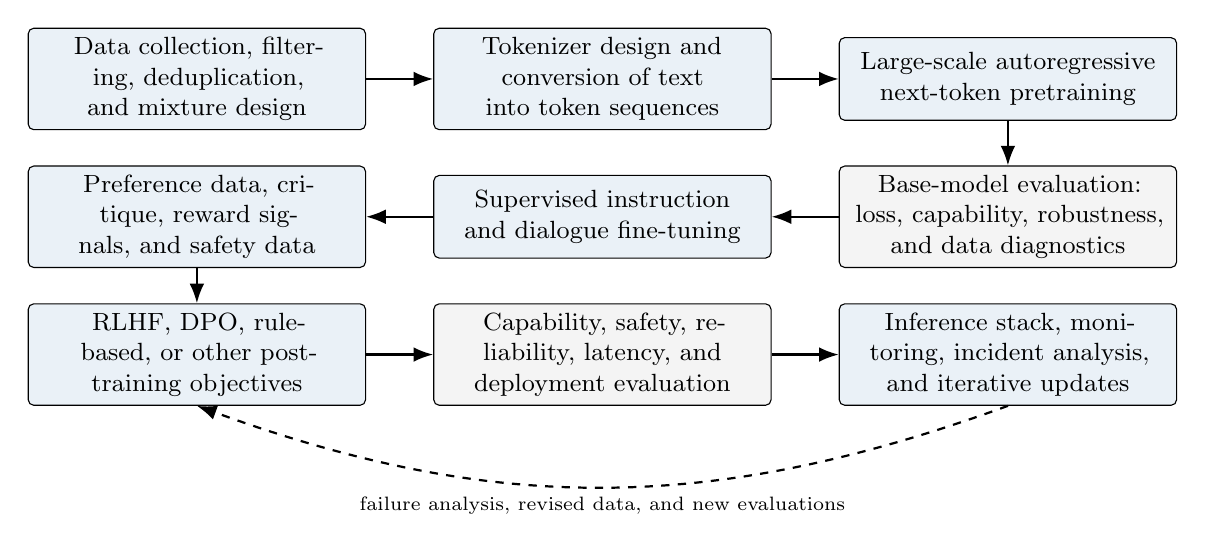
\begin{tikzpicture}[
  box/.style={draw,rounded corners=2pt,text width=4.05cm,minimum height=1.05cm,align=center,fill=SoftBlue,font=\small},
  eval/.style={draw,rounded corners=2pt,text width=4.05cm,minimum height=1.05cm,align=center,fill=SoftGray,font=\small},
  arrow/.style={-{Latex[length=2.5mm]},thick}
]
\node[box] (data) at (0,0) {Data collection, filtering, deduplication, and mixture design};
\node[box] (tok) at (5.15,0) {Tokenizer design and conversion of text into token sequences};
\node[box] (pre) at (10.30,0) {Large-scale autoregressive next-token pretraining};
\node[eval] (eval0) at (10.30,-1.75) {Base-model evaluation: loss, capability, robustness, and data diagnostics};
\node[box] (sft) at (5.15,-1.75) {Supervised instruction and dialogue fine-tuning};
\node[box] (pref) at (0,-1.75) {Preference data, critique, reward signals, and safety data};
\node[box] (post) at (0,-3.50) {RLHF, DPO, rule-based, or other post-training objectives};
\node[eval] (safe) at (5.15,-3.50) {Capability, safety, reliability, latency, and deployment evaluation};
\node[box] (serve) at (10.30,-3.50) {Inference stack, monitoring, incident analysis, and iterative updates};
\draw[arrow] (data)--(tok);
\draw[arrow] (tok)--(pre);
\draw[arrow] (pre)--(eval0);
\draw[arrow] (eval0)--(sft);
\draw[arrow] (sft)--(pref);
\draw[arrow] (pref)--(post);
\draw[arrow] (post)--(safe);
\draw[arrow] (safe)--(serve);
\draw[arrow,dashed] (serve.south) to[bend left=20] node[below,align=center,font=\scriptsize]{failure analysis, revised data, and new evaluations} (post.south);
\end{tikzpicture}
\caption{A simplified modern language-model development pipeline. Real systems iterate across stages and may use additional objectives, data sources, and safety layers.}
\label{fig:pipeline}
\end{figure}

\paragraph{Data and tokenization.}
Training begins with large corpora assembled from public, licensed, partnered, user-provided, trainer-generated, or synthetic sources. Data pipelines filter low-quality, duplicate, harmful, private, or otherwise unsuitable content, though no filter is perfect. A tokenizer maps text to discrete token identifiers. Modern tokenizers commonly represent frequent strings with single tokens and rare strings with multiple subword tokens. The vocabulary and segmentation influence sequence length, multilingual performance, code representation, and training efficiency.

\paragraph{Pretraining.}
For a token sequence $x_1,\ldots,x_T$, an autoregressive model with parameters $\theta$ is trained to maximize
\begin{equation}
  \log p_{\theta}(x_{1:T}) = \sum_{t=1}^{T} \log p_{\theta}(x_t \mid x_{<t}).
\end{equation}
Equivalently, training minimizes cross-entropy between the predicted next-token distribution and the observed next token. Over many examples, the model learns statistical regularities spanning syntax, style, world knowledge, code patterns, and problem-solving traces. Pretraining does not store a clean database of facts. It shapes a distributed conditional predictor whose behavior depends on the prompt.

\paragraph{Post-training.}
Supervised fine-tuning trains on demonstrations of desired behavior. Preference data compare candidate outputs, either through human labels, model-assisted labels, rule-based graders, or combinations. In an RLHF pipeline, a reward model predicts the preferred output and the policy is optimized against that signal, often with a penalty that limits departure from a reference model. Direct preference methods optimize pairwise preferences more directly. Post-training improves behavior that pretraining made possible, but can also introduce style biases, sycophancy, verbosity, reward hacking, or over-refusal.

\paragraph{Evaluation and deployment.}
A deployment pipeline evaluates capability, factuality, safety, robustness, tool use, latency, cost, and failure modes. The serving system adds inference kernels, batching, caching, routing, permissions, monitoring, and product-level safeguards. Product behavior therefore cannot be inferred from architecture alone.

\subsection{ChatGPT and GPT-3.5 as a public example}\label{sec:chatgpt-example}

The original ChatGPT release is a useful example because its high-level post-training sequence was publicly described. An initial dialogue model was trained with supervised fine-tuning: human trainers produced conversations playing both user and assistant roles, with access to model suggestions. For preference training, multiple model responses were sampled and ranked. A reward model was trained from those comparisons, and the policy was refined using PPO over several iterations \cite{openaichatgpt2022}. ChatGPT was described as fine-tuned from a model in the GPT-3.5 series.

Figure~\ref{fig:chatgpt} expresses that public sequence without claiming undisclosed architectural details.

\begin{figure}[H]
\centering
\resizebox{0.94\linewidth}{!}{%
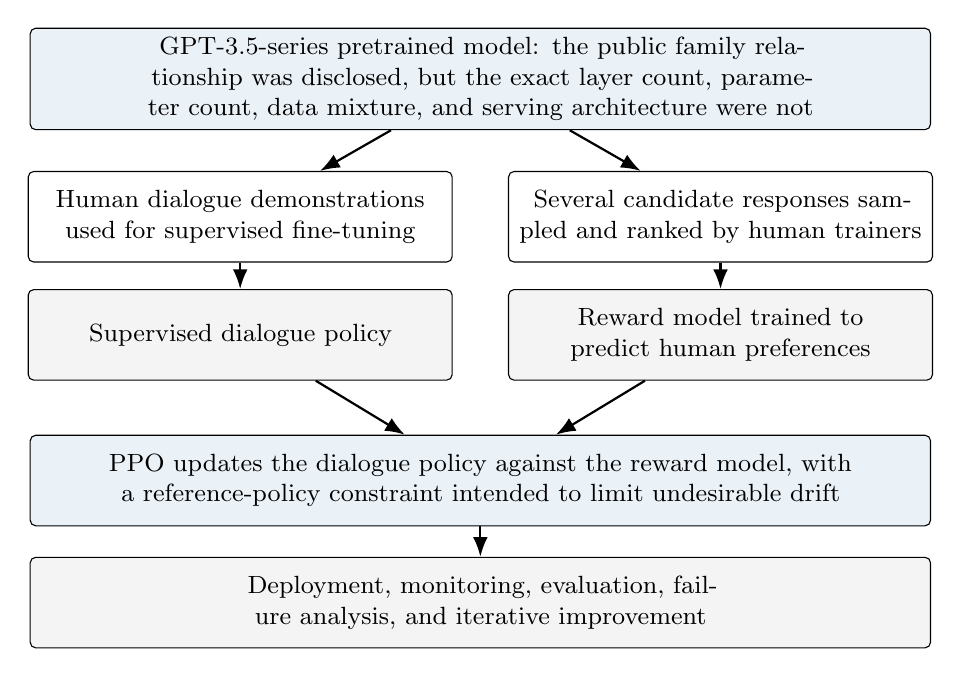
\begin{tikzpicture}[
  box/.style={draw,rounded corners=2pt,text width=5.15cm,minimum height=1.15cm,align=center,font=\small},
  wide/.style={draw,rounded corners=2pt,text width=11.2cm,minimum height=1.15cm,align=center,font=\small},
  arrow/.style={-{Latex[length=2.5mm]},thick}
]
\node[wide,fill=SoftBlue] (base) at (0,0) {GPT-3.5-series pretrained model: the public family relationship was disclosed, but the exact layer count, parameter count, data mixture, and serving architecture were not};
\node[box] (demo) at (-3.05,-1.75) {Human dialogue demonstrations used for supervised fine-tuning};
\node[box] (comp) at (3.05,-1.75) {Several candidate responses sampled and ranked by human trainers};
\node[box,fill=SoftGray] (sft) at (-3.05,-3.25) {Supervised dialogue policy};
\node[box,fill=SoftGray] (rm) at (3.05,-3.25) {Reward model trained to predict human preferences};
\node[wide,fill=SoftBlue] (ppo) at (0,-5.10) {PPO updates the dialogue policy against the reward model, with a reference-policy constraint intended to limit undesirable drift};
\node[wide,fill=SoftGray] (deploy) at (0,-6.65) {Deployment, monitoring, evaluation, failure analysis, and iterative improvement};
\draw[arrow] (base)--(demo);
\draw[arrow] (base)--(comp);
\draw[arrow] (demo)--(sft);
\draw[arrow] (comp)--(rm);
\draw[arrow] (sft)--(ppo);
\draw[arrow] (rm)--(ppo);
\draw[arrow] (ppo)--(deploy);
\end{tikzpicture}}
\caption{Publicly described ChatGPT training sequence. This figure does not infer undisclosed architectural or data details for GPT-3.5.}
\label{fig:chatgpt}
\end{figure}

The example demonstrates why model size alone is not a complete measure of assistant quality. OpenAI reported that a 1.3-billion-parameter InstructGPT model was preferred to a 175-billion-parameter GPT-3 model on evaluated prompts after human-feedback training \cite{openaiinstruct2022}. In summarization, a 1.3-billion-parameter human-feedback model outperformed a 12-billion-parameter supervised model in human preference judgments \cite{openaisummarize2020}. These comparisons concern particular tasks, data, and evaluation procedures. They do not imply that small models generally outperform large models.

\subsection{Decoder-only Transformer architecture}\label{sec:transformer}

Most GPT-style LLMs use a stack of decoder-only Transformer blocks. Figure~\ref{fig:transformer} shows a simplified architecture.

\begin{figure}[H]
\centering
\resizebox{0.90\linewidth}{!}{%
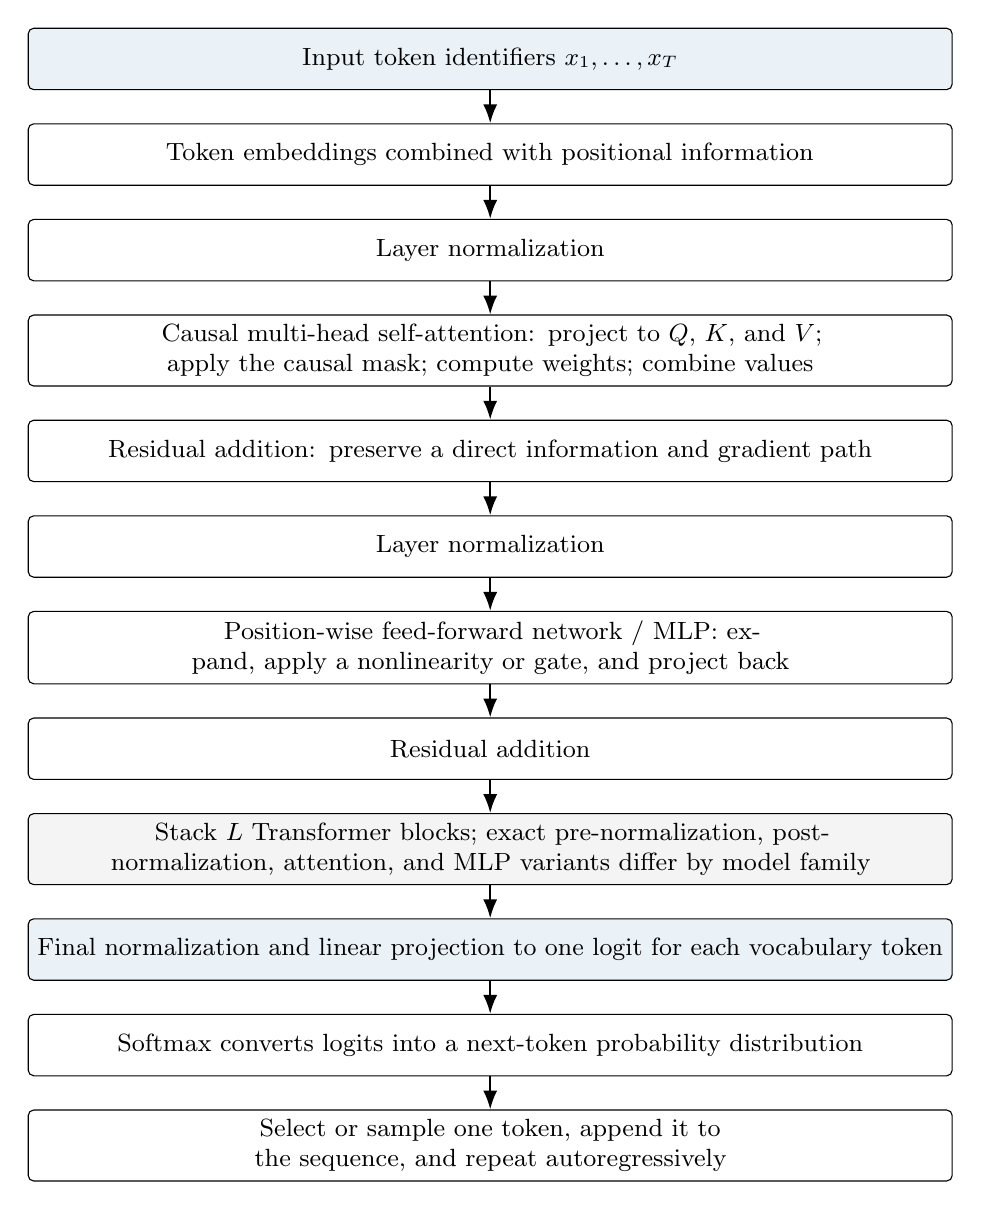
\begin{tikzpicture}[
  node distance=4.2mm,
  box/.style={draw,rounded corners=2pt,text width=11.5cm,minimum height=0.78cm,align=center,font=\small},
  arrow/.style={-{Latex[length=2.4mm]},thick}
]
\node[box,fill=SoftBlue] (tokens) {Input token identifiers $x_1,\ldots,x_T$};
\node[box,below=of tokens] (embed) {Token embeddings combined with positional information};
\node[box,below=of embed] (norm1) {Layer normalization};
\node[box,below=of norm1] (attn) {Causal multi-head self-attention: project to $Q$, $K$, and $V$; apply the causal mask; compute weights; combine values};
\node[box,below=of attn] (res1) {Residual addition: preserve a direct information and gradient path};
\node[box,below=of res1] (norm2) {Layer normalization};
\node[box,below=of norm2] (mlp) {Position-wise feed-forward network / MLP: expand, apply a nonlinearity or gate, and project back};
\node[box,below=of mlp] (res2) {Residual addition};
\node[box,below=of res2,fill=SoftGray] (repeat) {Stack $L$ Transformer blocks; exact pre-normalization, post-normalization, attention, and MLP variants differ by model family};
\node[box,below=of repeat,fill=SoftBlue] (out) {Final normalization and linear projection to one logit for each vocabulary token};
\node[box,below=of out] (soft) {Softmax converts logits into a next-token probability distribution};
\node[box,below=of soft] (sample) {Select or sample one token, append it to the sequence, and repeat autoregressively};
\draw[arrow] (tokens)--(embed);
\draw[arrow] (embed)--(norm1);
\draw[arrow] (norm1)--(attn);
\draw[arrow] (attn)--(res1);
\draw[arrow] (res1)--(norm2);
\draw[arrow] (norm2)--(mlp);
\draw[arrow] (mlp)--(res2);
\draw[arrow] (res2)--(repeat);
\draw[arrow] (repeat)--(out);
\draw[arrow] (out)--(soft);
\draw[arrow] (soft)--(sample);
\end{tikzpicture}}
\caption{Simplified decoder-only Transformer. Exact normalization order, activation functions, attention variants, position representations, and parameter sharing differ across model families.}
\label{fig:transformer}
\end{figure}

\subsubsection{Embeddings and position}

A token embedding matrix maps each token identifier to a vector in $\mathbb{R}^{d_{\text{model}}}$. Position information is then incorporated, for example through learned embeddings, sinusoidal encodings, rotary position embeddings, or related schemes. Without position, self-attention would treat the input largely as an unordered set. Position mechanisms let the model distinguish ``dog bites person'' from ``person bites dog'' and represent relative or absolute sequence order.

\subsubsection{Queries, keys, values, and causal attention}

For a layer input matrix $X\in\mathbb{R}^{T\times d_{\text{model}}}$, one attention head computes
\begin{align}
Q &= XW_Q, & K &= XW_K, & V &= XW_V,\\
A &= \operatorname{softmax}\left(\frac{QK^{\top}}{\sqrt{d_h}} + M\right),\\
\operatorname{Attention}(X) &= AV,
\end{align}
where $d_h$ is the head dimension and $M$ is a causal mask assigning a very negative value to prohibited future positions. A query describes what the current position is seeking; keys describe how earlier positions can be matched; values carry the information combined according to the attention weights. These are functional interpretations, not human-readable semantic labels fixed for every head.

Multi-head attention computes several such transformations, concatenates their outputs, and applies an output projection:
\begin{equation}
\operatorname{MHA}(X)=\operatorname{Concat}(H_1,\ldots,H_{n_h})W_O.
\end{equation}
Different heads can represent different interactions, though a head is not guaranteed to correspond to a single clean concept.

\subsubsection{Residual paths, normalization, and the MLP}

Residual connections add a sublayer's output to its input. They improve optimization and let information travel through deep stacks without requiring every layer to reconstruct the full representation. Layer normalization stabilizes activation scale. Architectures differ between pre-normalization and post-normalization orders.

The feed-forward network applies a nonlinear transformation independently to each position, typically expanding to a larger hidden dimension and projecting back:
\begin{equation}
\operatorname{MLP}(x)=W_2\,\sigma(W_1x+b_1)+b_2,
\end{equation}
with an activation such as GELU or a gated variant. Attention mixes information across positions; the MLP transforms the representation at each position. Both are central.

\subsubsection{Output projection and autoregressive generation}

After the final block, a linear projection maps the hidden state to one logit per vocabulary token. Softmax turns logits into probabilities. A decoding rule then chooses the next token. Greedy decoding takes the highest-probability token; temperature, top-$k$, top-$p$, or other sampling methods alter the distribution. The chosen token is appended to the context and the process repeats until a stop condition is reached.

This process explains both capability and fragility. The model can synthesize patterns over long contexts, but every generated token also becomes context for later tokens. Early misinterpretations can therefore become self-reinforcing. Explicit contracts, checks, and tool observations can interrupt that trajectory.

\subsection{Prefill, decoding, and the KV cache}\label{sec:kv-cache}

Inference has two main phases. During \emph{prefill}, the model processes the supplied prompt and computes hidden states for all positions. During \emph{decode}, it generates one or a small number of new tokens at a time. Naively recomputing attention keys and values for every previous token on every decode step would be wasteful. The serving system therefore stores each layer's previous keys and values in a KV cache.

For batch size $B$, sequence length $S$, $L$ layers, $n_{kv}$ key/value heads, head dimension $d_h$, and $b$ bytes per stored scalar, an approximate cache size is
\begin{equation}
M_{KV}\approx 2BSLn_{kv}d_hb.
\end{equation}
The factor of two accounts for keys and values. With $L=32$, $S=8192$, $n_{kv}=8$, $d_h=128$, $b=2$, and $B=1$, the cache is approximately one GiB. Four sequences require approximately four GiB before allocator overhead and other model state. Standard multi-head attention with 32 KV heads would require roughly four times as much cache for the same dimensions. Multi-query and grouped-query attention reduce the number of KV heads and therefore reduce serving memory \cite{shazeer2019,ainslie2023}. FlashAttention improves attention IO behavior, while PagedAttention improves memory allocation for variable-length serving workloads \cite{dao2022,kwon2023}.

The KV cache has an important but limited implication for workflow design. It makes repeated use of previous context computationally cheaper than recomputing it. It does \emph{not} decide which instruction is important, infer that a user is professional, or reward a structured file layout. Structured context can improve outcomes because it reduces ambiguity, improves placement of decisive information, and narrows the action space. Those are semantic and interface effects, not direct consequences of cache mechanics.

\subsection{Three simplified model-development regimes}\label{sec:model-regimes}

For workflow design, it is useful to distinguish three simplified regimes. They are not exhaustive categories and should not be treated as a law of model development.

\begin{table}[H]
\centering
\caption{Three simplified development regimes relevant to model allocation.}
\begin{tabularx}{\textwidth}{P{0.20\textwidth}P{0.24\textwidth}Y Y}
\toprule
\textbf{Regime} & \textbf{Training emphasis} & \textbf{Potential strength} & \textbf{Potential weakness} \\
\midrule
Parameter-heavy / undertrained & Very large parameter count relative to the available training tokens or compute allocation. & Broad representational capacity and possible frontier capability if sufficiently trained. & Expensive inference; parameters may be underutilized; a smaller better-trained model can outperform it at fixed compute. \\
Compute-balanced & Parameters and training tokens scaled together under a compute budget. & Strong general performance per unit of training compute, as illustrated by compute-optimal scaling work. & Still expensive for high-volume deployment; ``balanced'' depends on objective, data quality, and serving costs. \\
Smaller, data-heavy, specialized, or distilled & Fewer parameters with more training tokens, curated task data, strong post-training, distillation, or a combination. & Lower inference cost and latency; attractive for repeated bounded subagent tasks when competence is sufficient. & Lower ceiling on some complex tasks; specialization can reduce breadth; distillation may transfer or amplify teacher errors. \\
\bottomrule
\end{tabularx}
\end{table}

The subagent implication is conditional. Inference-aware scaling work shows that, under sufficiently high expected serving demand, training a smaller model for longer can minimize total training-plus-inference cost, and quality can continue to improve at unusually high token-to-parameter ratios \cite{sardana2024}. This supports the economic logic of compact specialist workers, but not a universal quality claim. A smaller model is an appropriate subagent when the assignment is bounded, the required context is limited, the output can be checked, and evaluation demonstrates acceptable performance. Low cost alone is not a sufficient allocation criterion. Main should match model capability to task difficulty and escalate when the worker exhibits repeated errors, uncertainty, or scope drift.

\subsection{Model-family lineage and inter-model communication}\label{sec:model-lineage}

A model family can share a provider, generation label, architecture, tokenizer, pretraining corpus, post-training recipe, teacher outputs, or product interface. These relationships are distinct. Shared branding alone does not specify which components are common, while explicit distillation can transfer capabilities without reproducing the teacher's complete behavior. Table~\ref{tab:family-lineage} summarizes public disclosures for representative families.

\begingroup
\small
\setlength{\tabcolsep}{4pt}
\begin{longtable}{P{0.16\textwidth}P{0.31\textwidth}P{0.22\textwidth}P{0.23\textwidth}}
\caption{Public lineage signals in selected model families.}\label{tab:family-lineage}\\
\toprule
\textbf{Family} & \textbf{Disclosed transfer} & \textbf{Shared-data disclosure} & \textbf{Allocation note} \\
\midrule
\endfirsthead
\toprule
\textbf{Family} & \textbf{Disclosed transfer} & \textbf{Shared-data disclosure} & \textbf{Allocation note} \\
\midrule
\endhead
OpenAI GPT-5.6 & Sol, Terra, and Luna are capability tiers; no Sol-to-Terra/Luna teacher relation is disclosed \cite{openai56release2026}. & Exact overlap: ND. & Common interface may reduce friction; test correlated error. \\
Anthropic Claude & Opus, Sonnet, and Haiku are family tiers; teacher relation: ND \cite{anthropictransparency2026}. & Broad categories only. & Shared conventions help formatting; tier behavior can differ. \\
Qwen3 & Strong-to-weak transfer from larger to smaller models \cite{qwen3report2025}. & Family corpus described broadly. & Compact workers are plausible after task evaluations. \\
DeepSeek-R1 & R1-generated samples train Qwen/Llama distill checkpoints \cite{deepseekr1}. & Student bases retain their own pretraining. & Transfer can cross families. \\
Gemini 1.5 & Flash distilled from Pro \cite{googleflash2024}. & Exact overlap: ND. & Direct teacher--student example. \\
Llama 3.2 & Pruning plus teacher logits from larger Llama models \cite{metallama32}. & Family recipe described broadly. & Compact workers still require validation. \\
\bottomrule
\end{longtable}
\vspace{-2mm}
\noindent\footnotesize ND = not disclosed in the cited sources; it is not evidence of absence.
\endgroup

The research on inter-model communication suggests three operational conclusions. First, models can infer interlocutor identity and recognize same-family peers from output patterns \cite{choi2025interlocutor}. Second, evaluator models can recognize and prefer their own generations, creating a risk of biased self-review \cite{panickssery2024}. Third, post-training recipe and partner identity may predict interactive behavior more strongly than the provider-family label alone \cite{zhang2026posttraining}. Family similarity can therefore improve protocol compatibility while simultaneously increasing correlated errors and mutual over-acceptance.

The workflow should use family relationships as one allocation variable rather than a guarantee. Same-family Main and worker configurations may reduce protocol translation in bounded implementation because the models can share product conventions, tool schemas, and response formats. This is an operational hypothesis rather than a universal performance result. Independent verification and broad research may benefit from cross-family or separately trained diversity, provided that outputs are normalized into a common evidence schema. Distillation status, shared training data, and family identity should be recorded when publicly disclosed, but task-specific evaluation remains the decisive criterion.



\section{Rationale for the Current Workflow Architecture}\label{sec:rationale}

\subsection{Prompts as conditional interfaces}\label{sec:conditional-interface}
An instruction-following model does not receive the user's intention directly. It receives a context containing prompts, retrieved files, tool schemas, prior outputs, environment observations, and system instructions, then conditions its next action on that mixture. A durable workflow improves this interface by externalizing state, narrowing role-specific context, and making acceptance observable. The prompt is therefore an interface to a larger state machine rather than a self-sufficient specification.

A practical consequence follows. Prompt quality cannot be assessed only by prose style. A good execution prompt is one whose outcome, state, dependencies, authority, evidence, and return contract are aligned with the active DIC and actual executor surface. This is why EPS prompts are generated or refreshed against current state rather than frozen forever merely because an earlier template was well written.

\subsection{Context engineering and selective context construction}\label{sec:context-rationale}
Long context is capacity, not a guarantee of uniform attention or correct interpretation. Main should retain the Primary Aim, binding decisions, compact evidence, and unresolved material questions. Theory should receive the exact formal problem and relevant source/evidence objects. Experiment should receive the estimand, protocol, data/seed identities, and frozen controls. Workers should receive one bounded work package plus the files needed for that package. Verifiers should receive decisive artifacts and acceptance criteria rather than the implementation agent's full persuasive narrative.

The package therefore prefers \emph{selective sufficiency}: every role receives enough information to make its next decision, but not the entire history of the project. Durable files, hashes, manifests, compact handoffs, and on-demand retrieval preserve continuity without forcing the next model invocation to ingest all previous activity.

\subsection{Hierarchical refinement instead of one enormous research prompt}\label{sec:hierarchy-rationale}
A request such as ``research the literature, design the method, implement it, run the experiments, analyze the result, write the paper, and verify everything'' conflates several timescales and evidence classes. AI Native Workflow refines intent through
\[
\text{Goal}\to\text{Plan}\to\text{Phase}\to\text{DIC}\to\text{EPS}\to\text{Prompt/Run}\to\text{Action}.
\]
The hierarchy protects durable meaning while allowing lower levels to be regenerated as evidence changes. Goal and Plan are programme-scale. A Phase is one coherent milestone. Its single DIC is repair-stable unless the scientific contract itself changes. EPS is disposable and may be regenerated many times. Individual prompts/runs and actions are attempt-local.

This makes hierarchical planning practically available within current persistent-chat and coding-agent settings. It does not claim a new planning algorithm; it specifies where planning artifacts live, who owns them, how they are refined, and how evidence changes later execution.

\subsection{One DIC per Phase as both contract and compression interface}\label{sec:dic-rationale}
Each Phase has exactly one multi-view DIC. Its three required views are:
\begin{itemize}
\item \texttt{README.md}: orientation, Primary Aim, salience structure, authority, read order, and current context;
\item \texttt{REQUESTS.md}: prioritized observable outcomes and verifier-decidable acceptance targets;
\item \texttt{PLAN.md}: durable execution topology---dependencies, sequence, parallel branches, merge nodes, evidence gates, and conditional review/repair paths.
\end{itemize}
Optional views such as architecture, test matrix, claim map, data contract, or venue contract are added only when they reduce ambiguity.

A DIC is not a verbose transcript of everything the agents know. It is the smallest durable human-readable surface that preserves what the Phase means and what evidence can close it. This distinction matters for human attention: a researcher should inspect one coherent contract rather than reconstruct meaning from a pile of prompt logs.

\subsection{Main as semantic center; coding-agent Orchestrator as operational center}\label{sec:orchestrator-translation}
Main is a persistent user-facing chat session. It recovers durable state, interprets the user's objective, protects the Primary Aim, decides when Theory, Experiment, or Research support is needed, authors the whole-Phase DIC, integrates specialist returns, and handles material adjudication or closure. Main should not accumulate terminal noise or manage each execution prompt.

The Orchestrator is a repository-aware coding-agent execution surface such as Codex or Claude Code. It consumes the approved DIC and Main-authored initial EPS, validates dependency readiness, compiles prompts to the actual executor/model surface, launches bounded Workers or subagents, integrates returns, records evidence, performs bounded repair, and dispatches verification. Ordinary execution failure may create a superseding repair EPS under the unchanged DIC.

This separation is both an authority control and an attention control. It keeps semantic decisions away from noisy implementation traces and keeps runtime agents from silently reinterpreting the user's scientific objective while trying to make execution succeed.

\subsection{Core scientific workstreams and research as a capability}
The normal persistent scientific workstreams are Main, Theory, and Experiment. Main is always present. Theory is activated for formal reasoning, counterexamples, theorem/novelty analysis, and conceptual interpretation. Experiment is activated for estimands, benchmark design, frozen protocols, statistics, and empirical interpretation. They are not three mandatory agents in every Phase.

Research is a cross-cutting decision-support capability. A high-level path is
\[
\text{Main question}\to\text{Research}\to\text{Main reconciliation}\to\text{binding DIC decision}.
\]
Research returns primary-source evidence, disagreement, uncertainty, and implementation implications. It does not gain mutation authority or count as implementation evidence merely because its recommendation is persuasive.

\subsection{Allocation of bounded work to subagents}\label{sec:subagent-allocation}
Subagents are useful when work is independent enough to isolate context and recombine through explicit evidence: disjoint repository inspection, alternative proof attacks, literature/novelty scans, independent experiment branches, or replication. They should not be created merely to increase activity. Sibling subagents should normally be read-only or have disjoint write ownership; shared-state mutation without a declared merge procedure is a common source of silent conflict.

Prompt decomposition follows the same principle. Prefer one primary outcome and one to three tightly coupled work packages per prompt. Split when parts have different dependencies, evidence types, expertise, tools, write owners, parallelism, or retry semantics. Do not split into one prompt per shell command.

\subsection{Constraint--objective inversion and salience control}
Long-horizon research can fail even when every local action is competent. Defensive drift occurs when constraints become the effective objective. Salience flattening occurs when every idea is treated as equally worthy. Main and the DIC therefore maintain an explicit Primary Aim, supporting questions, constraints, optional branches, non-goals, and deferred work. Theory and Experiment are instructed to strengthen or falsify the Primary Aim rather than accumulate tangential work simply because it is available.

This is also a writing and reporting principle. A good research programme is not one in which every paragraph, theorem, caveat, or benchmark receives equal weight. The workflow should preserve a visible hierarchy of importance so that machine-generated breadth does not dilute the scientific center of gravity.

\subsection{Evidence reporting and uncertainty calibration}\label{sec:evidence-reporting}
Completion is linked to named evidence rather than fluent prose. Evidence classes are separated: proxy, smoke/fixture, pilot, locked/confirmatory, formal proof, independent verification, and external outcome. A smoke test may establish that a path runs; it does not establish a scientific claim. A verifier may confirm that evidence satisfies the declared predicate; it does not make the evidence statistically independent or epistemically infallible.

Negative results and failed branches remain visible. A system that silently deletes inconvenient failures makes the final narrative easier to read but less trustworthy. The human-facing report can remain concise because raw evidence stays addressable by path and hash.

\subsection{Action-space design, security, and safe defaults}\label{sec:action-space}\label{sec:sandbox}
The workflow distinguishes available capability from authorized action. Repository writes, external systems, purchases/paid compute, credentials, destructive operations, public release, and submission have separate authority boundaries. Sandboxing, least privilege, exact target identity, dry runs, snapshots, and post-action checks remain defense-in-depth controls. The runtime is a coordination layer rather than a security boundary.

\subsection{Why human-attention intensity is a better operational target}
Raw elapsed time is a poor universal objective. Parallelism can reduce wall-clock time while increasing aggregate inference. Strong verification can make a run slower but reduce downstream rework. A compact DIC may require more upfront structuring but reduce later reconstruction. Human-attention intensity captures the intended trade more directly: move low-value supervisory work into the machine while preserving high-value judgement.

This quantity should not be interpreted as a universal productivity metric. Human attention is difficult to observe, progress weights are project-specific, and expertise changes what counts as a costly intervention. Comparisons must therefore freeze task definitions, progress milestones, intervention taxonomy, and measurement procedure before evaluation.


\section{Current Operational Architecture}\label{sec:current-architecture}

\subsection{Distribution package versus operative runtime}
The full development distribution contains the technical report, research/theory artifacts, experiment protocols, workshop submissions, slides, validation history, and versioned tracking state. These files support development and publication. They are not all runtime instructions. The operative installation boundary is one directory:
\begin{lstlisting}[style=workflow]
project/
  .ai-workflow/
  AGENTS.md                 # project-local, if present
  agent.manifest.yaml       # project-local, if present
  phases/                   # project-local durable execution state
  src/ tests/ ...           # ordinary repository files
\end{lstlisting}
Only \texttt{.ai-workflow/} is copied from the workflow distribution into a target repository. The surrounding distribution is general storage for development of the workflow itself.

\subsection{Canonical hierarchy and persistence}
\begin{table}[H]
\centering\small
\begin{tabularx}{\textwidth}{@{}l l Y Y@{}}
\toprule
Level & Typical lifetime & Primary question & Persistence rule\\
\midrule
Goal & programme & What overall outcome matters? & durable\\
Plan & several phases & What milestones and dependencies define the programme? & durable, human-visible\\
Phase & milestone & What coherent result should be established now? & durable\\
DIC & Phase & What does this Phase mean and what evidence closes it? & durable across ordinary repair\\
EPS & attempt & How will ready DIC nodes be realized now? & disposable/versioned\\
Prompt/Run & bounded invocation & What does this executor do now? & logged\\
Action & primitive & What tool/edit/search/test occurs? & evidence-linked\\
\bottomrule
\end{tabularx}
\caption{Current refinement hierarchy.}
\end{table}

Durability decreases down the hierarchy. Ordinary execution failure should normally create a fresh EPS or prompt/run rather than rewriting higher semantic state. Replanning crosses upward only when the current DIC cannot honestly deliver the Primary Aim under its acceptance/authority boundary.

\subsection{Plan and Phase semantics}
A Plan is the programme-scale strategic DAG. It may authorize multiple ordinary Phases between human checkpoints. A Phase is a coherent milestone, not normally a human approval ceremony. Main proposes and records the next whole Phase under the approved Plan. Periodic checkpoints or material escalations return to the human when scientific meaning, authority, risk, or external responsibility changes.

This distinction reduces human coordination attention. The human should not be asked to approve every executor prompt merely because the runtime has decomposed a Phase into many actions.

\subsection{The single multi-view DIC}
Every Phase has exactly one DIC. Its three Core views are required and complementary rather than sequential:
\begin{lstlisting}[style=workflow]
DIC/
  README.md       # orientation + Primary Aim + authority + current context
  REQUESTS.md     # prioritized outcomes + acceptance/evidence targets
  PLAN.md         # durable dependency / sequence / parallelism graph
\end{lstlisting}
\texttt{PLAN.md} explicitly represents the prompt/execution topology planned by Main: sequence, parallel groups, dependencies, merge points, subagent branches, integration barriers, verification gates, and conditional repair/review branches. It is not itself the runtime prompt text. Main maps those durable nodes into the initial EPS/prompt graph; Orchestrator may later issue bounded repair EPS revisions when execution-local evidence requires them.

\subsection{Primary Aim and request salience}
The DIC should expose one Primary Aim in a single sentence. Requests are classified as primary, supporting, optional, or deferred. A Phase with ten equally weighted objectives is usually underspecified: either the Primary Aim is missing or the work should be split into separate Phases. The DIC therefore acts as a salience contract as well as an execution contract.

A useful human-facing review asks:
\begin{enumerate}
\item If all optional branches vanished, would the Phase still establish its Primary Aim?
\item Could a constraint be mistaken for the objective?
\item Is there a single piece of decisive evidence that would materially change the next decision?
\item Does every primary request have a verifier-decidable acceptance condition?
\end{enumerate}

\subsection{EPS semantics}
An EPS is an executable realization of DIC plan nodes for one attempt. \emph{Main authors the initial EPS/prompt graph} together with the Phase handoff. It records plan-node identity, dependencies, bounded prompt bodies, intended executor role, parallel groups, subagent flags, evidence requirements, and stop conditions. Before dispatch, Orchestrator validates this graph and compiles the prompt wording/tool-facing details for the actual model and execution surface. Multiple EPS attempts may realize the same unchanged DIC after new evidence arrives.

This separation is essential for local recovery. If a coding prompt is defective, or one implementation attempt fails, the scientific contract should not be rewritten as though the failed execution never existed. The Main-authored initial EPS remains provenance; Orchestrator may create a bounded superseding repair EPS under the same DIC.

\subsection{Model-tuned prompt compilation}
Generic templates are scaffolds, not final prompts. Before dispatching a model-executed EPS node, Orchestrator resolves the actual execution model and surface and applies the appropriate prompt guidance. The conceptual compiler is:
\[
\begin{aligned}
\text{DIC + current evidence}
&\to \text{PROMPTING\_CORE}\\
&\to \text{provider/model overlay}\\
&\to \text{surface overlay}\\
&\to \text{bounded execution prompt}.
\end{aligned}
\]
The final prompt should state one primary outcome, success/evidence criteria, relevant state/dependencies, hard constraints, authority boundaries, outputs, checks, repair/stop behavior, and return contract. Duplicated or irrelevant instructions introduced by composition are removed before dispatch.

\subsection{Coding-agent Orchestrator protocol}
The coding-agent Orchestrator executes the whole Phase. Its normal loop is:
\begin{enumerate}
\item recover root, Phase, DIC, and current EPS/evidence state;
\item validate authority and readiness;
\item identify dependency-ready DIC plan nodes;
\item choose direct execution versus bounded subagent decomposition;
\item tune prompts to actual model/surface;
\item execute independent branches concurrently where write ownership and interfaces permit;
\item integrate returns at declared merge nodes;
\item reject incomplete evidence or create bounded repair EPS attempts;
\item dispatch verification at declared boundaries;
\item return material replan/escalation to Main rather than silently changing the DIC;
\item produce a durable handoff at Phase closure.
\end{enumerate}

\subsection{Bounded Workers and subagents}
A Worker/subagent receives one complete bounded task, relevant files, allowed/forbidden scope, evidence requirements, and return contract. It does not gain Phase authority by being capable of additional work. Sibling write ownership should be disjoint unless a parent merge procedure is explicit. Independent read-only analysis can be parallelized more aggressively.

The parent remains responsible for integration. Worker completion is not Orchestrator integration; integration is not verification; verification is not human approval for external consequences.

\subsection{Research, Theory, and Experiment integration}
A Main-led research programme may follow:
\begin{lstlisting}[style=workflow]
Main question
  -> Research (if external evidence can change the decision)
  -> Main reconciliation
  -> Theory and/or Experiment specialist work
  -> Main whole-Phase DIC + initial EPS/prompt graph
  -> coding-agent Orchestrator validation / execution
  -> evidence
  -> Main reconciliation / closure / next Phase
\end{lstlisting}
Theory and Experiment may operate in parallel when their evidence is genuinely separable. Research may be requested by Main or by a specialist workstream, but any binding change to method, protocol, claim, or Phase meaning returns through Main.

\subsection{Verification outcomes}
Verification is a control signal rather than a terminal score. The canonical outcomes are:
\begin{description}
\item[accept] current evidence satisfies the acceptance predicate;
\item[repair] the DIC remains valid but execution/evidence within its boundary must be corrected;
\item[replan] the current route/contract cannot honestly deliver and a higher-level plan change is required;
\item[escalate] human/material authority is required.
\end{description}
This four-way distinction prevents the common failure in which every negative result is treated as another local retry.

\subsection{Evidence and recovery}
Actions bind to evidence paths and version identities. If a repaired source changes declared keys, only the declared dynamic impact cone must be invalidated under the locality assumptions formalized later. Unaffected evidence is retained rather than discarded merely because another branch failed. Conversely, hidden dependencies invalidate the guarantee; incomplete declarations are therefore a scientific and engineering risk, not merely a bookkeeping defect.

\subsection{Human-facing Main status}
Main's visible status should remain much smaller than the runtime graph. At Phase planning/reconciliation it should normally expose only:
\begin{table}[H]\centering\small
\begin{tabularx}{\textwidth}{@{}lY@{}}\toprule
Field & Human-facing meaning\\\midrule
Plan / Phase & current programme milestone\\
Primary Aim & central result the Phase exists to establish\\
Core workstreams & whether Main, Theory, Experiment are active\\
Research & not needed / requested / returned / integrated\\
DIC & one active DIC; Core three views complete/incomplete\\
DIC plan & concise durable sequence/parallelism summary\\
Initial EPS & Main-authored first executable prompt graph; ready/not ready\\
Evidence target & decisive evidence needed for closure\\
Human gate & none, or the exact material decision required\\
\bottomrule\end{tabularx}
\caption{Compact Main-facing status.}
\end{table}
The human should not be asked to monitor repair-EPS counts or worker logs unless those details become material evidence; Main should nevertheless be able to show that the initial EPS/prompt graph exists and is ready for handoff.

\subsection{Current-state authority}
Package state overrides chat memory. A fresh session should reconstruct the project by reading canonical files rather than relying on the previous conversation's narrative. The development distribution similarly separates current truth, future work, and history: \texttt{CURRENT\_STATE.md} describes what is true now; \texttt{ROADMAP.md} describes future work; \texttt{CHANGELOG.md} records history.


\section{Decision Rationale and Attention Economics}\label{sec:decision-rationale}

\subsection{Why Main is persistent chat}
Persistent chat is well suited to semantic continuity, clarification, synthesis, and material judgement. Main benefits from seeing the evolution of the user's objective but should not accumulate noisy terminal histories. Repository state remains the authority, so a new Main can recover if the original chat becomes unavailable or overloaded.

\subsection{Why the Orchestrator is specifically a coding-agent surface}
Repository execution has different requirements from semantic planning: file discovery, shell commands, patches, tests, artifact creation, environment feedback, and repeated local repair. Current coding-agent surfaces are designed for exactly these loops. Treating Orchestrator as a coding-agent session rather than another general planning chat reduces role ambiguity and makes the machine/human boundary legible.

\subsection{Why Research is explicit but not a permanent role}
External research is load-bearing only when it can change a decision. Requiring a standing Researcher for every Phase creates ceremony and context overhead; hiding research entirely makes it easy to forget that external evidence is available. The compromise is a first-class capability with an explicit Main decision gate. The returned report is advisory until Main records the binding implication.

\subsection{Why one DIC rather than sequential contracts}
Several sequential DICs inside one Phase would blur the distinction between durable meaning and execution steps. The single multi-view DIC provides one semantic anchor; its \texttt{PLAN.md} can still contain arbitrarily rich sequence, parallelism, branch, and merge structure. This is easier for humans to review and makes it possible to distinguish repair of execution from change of intent.

\subsection{Why the execution graph lives in DIC/PLAN.md}
The execution graph is part of what Main is planning: which scientific/technical work depends on what, what may run in parallel, what must merge before claims can advance, and where verification belongs. Hiding this entirely inside EPS would make the durable contract unable to explain the intended route. Conversely, storing actual prompt text and every runtime retry in \texttt{PLAN.md} would make the DIC unstable. The durable graph therefore names semantic plan nodes; EPS records their current operational realization.

\subsection{Why Main authors the initial EPS and why EPS remains disposable}
Execution conditions change: repositories evolve, tools fail, model availability changes, one branch returns negative evidence, or a prompt proves defective. Regenerating EPS lets the runtime adapt without rewriting history or weakening the approved Primary Aim. Versioned supersession also preserves provenance for later audit.

\subsection{Why prompts are smaller than phases}
A Phase may contain theory, literature, implementation, experiments, statistics, and paper changes. A single executor prompt spanning all of them is difficult to retry, hard to verify, and likely to mix evidence classes. Bounded prompts create local failure semantics and allow safe parallelism. However, excessive micro-prompting can waste context and integration effort. The split criterion is semantic: dependency, evidence, expertise, write ownership, or failure boundary---not individual shell commands.

\subsection{Why subagent use is explicit}
Subagent parallelism can reduce critical-path time and isolate contexts, but it can also multiply inconsistent interpretations and write conflicts. The Orchestrator must therefore actively consider subagents while retaining a bias toward direct execution for simple sequential work. Every subagent must have a parent integration point and bounded authority.

\subsection{Why DICs should become more readable as execution grows}
A common anti-pattern is proportional reporting: twice as many agent actions produce twice as much human-facing prose. That makes human attention scale with machine activity. AI Native Workflow instead treats reports as indexes into evidence and DICs as compressed decision surfaces. Raw artifacts remain available, but the human-facing layer emphasizes decisions, decisive evidence, unresolved questions, and material exceptions.

\subsection{Why the Primary Aim is explicit}
Long AI-assisted research can become surprisingly flat. Every caveat, alternative, side theorem, and benchmark may look locally valuable. Explicit salience prevents this breadth from erasing the project's main scientific question. The Primary Aim also provides a reference for deciding whether optional work should continue: an extension that neither strengthens nor falsifies the central claim is a candidate for deferral.

\subsection{Why defensibility is a constraint rather than the objective}
Adversarial review is useful, but repeated hostile audits can create constraint--objective inversion. The correct optimization problem is closer to ``find the strongest correct result subject to evidence and claim constraints'' than ``minimize all possible criticism.'' The workflow keeps correctness, safety, and evidence as hard boundaries while allowing ambition inside them.

\subsection{Why human attention, not tokens, is the principal coordination quantity}
Token counts and model calls measure machine resource use, not the researcher's supervisory burden. Wall-clock time conflates useful parallelism, queueing, model latency, and human waiting. Human attention is closer to the scarce resource the workflow is designed to reallocate. Evaluation should therefore record intervention classes, durations where feasible, manual routing/context-transfer events, reconstruction episodes, and the scientific materiality of interventions alongside conventional compute metrics.

\subsection{Why attention reduction is not automatically good}
A system can reduce human attention by hiding problems. The attention objective is therefore constrained by verified progress and false-acceptance outcomes. A workflow that requires little supervision but produces unsupported research should score poorly. The denominator in $\rho_H$ is verified progress rather than raw activity or number of generated artifacts.

\subsection{Why concise reports do not imply missing evidence}
The detailed evidence belongs in logs, artifacts, results, research records, verification outputs, and experiment manifests. Human reports summarize what changed and point to decisive evidence. This mirrors a broader separation between data plane and control plane: machine evidence can be large while the human control surface remains small.


\section{Operational Use of AI Native Workflow}\label{sec:operational-use}

\subsection{Adoption paths}
Researchers may adopt the workflow at three levels:
\begin{enumerate}
\item \textbf{Use the full runtime}: copy \texttt{.ai-workflow/} into the repository and follow the Main/Orchestrator path.
\item \textbf{Adapt selected architecture}: keep the existing tool stack while adding explicit separation between Phase, DIC, and EPS, Research reconciliation, or verification gates.
\item \textbf{Adopt individual mechanisms}: for example one multi-view DIC per research milestone, dependency-aware repair, Primary Aim/salience labels, or model-tuned prompt compilation.
\end{enumerate}
The workflow is a reference operating model, not a requirement to abandon existing project conventions.

\subsection{Starting from an existing informal workflow}
A common starting point is already something like:
\begin{lstlisting}[style=workflow]
ChatGPT / Claude persistent chat     -> planning and interpretation
Deep Research / browser              -> literature and novelty
Codex / Claude Code                  -> implementation and experiments
another chat                         -> analysis and paper writing
\end{lstlisting}
The upgrade is to externalize state and ownership. The researcher starts one persistent Main session, gives it the repository with \texttt{.ai-workflow/}, and asks it to recover current state rather than reconstructing the project manually. Main then proposes the next whole Phase and its DIC.

\subsection{Main session protocol}
At the start of a Main session:
\begin{enumerate}
\item read \texttt{.ai-workflow/docs/CORE.md} and \texttt{MAIN.md};
\item inspect project-local authority files and runtime state;
\item read the active Plan, Phase, DIC Core views, prior verified handoff, and unresolved material decisions;
\item preserve exact user input separately from Main's interpretation;
\item identify the Primary Aim and detect any defensive drift or salience flattening;
\item decide whether external Research, Theory, or Experiment work can materially improve the next decision;
\item author or revise the single whole-Phase DIC;
\item present the compact Phase checklist for human correction;
\item hand the whole Phase to the coding-agent Orchestrator when the DIC is ready.
\end{enumerate}
Main should not present a second chat-level execution prompt graph: the graph already belongs in \texttt{DIC/PLAN.md}.

\subsection{Research pass}
A Research request should name the exact decision it informs. Useful forms include novelty audit, benchmark/regime search, official specification lookup, method comparison, or literature-based falsification. The return should include an executive conclusion, source hierarchy, competing evidence, uncertainty, one ranked recommendation with fallback, and exact implications for DIC planning. Research output is not automatically binding and must not claim an implementation or experiment has occurred.

\subsection{Theory workstream}
Theory receives a bounded scientific question and the evidence needed to reason about it. For material claims, separate positive derivation, hostile audit, and novelty comparison where useful. Theory returns the strongest correct central statement, assumptions, counterexamples, and which side results are actually load-bearing. It should not turn every possible lemma into a permanent research branch.

\subsection{Experiment workstream}
Experiment freezes estimands, controls, benchmark design, seed/data namespaces, evidence ceilings, and analysis plans before confirmatory runs. Screening, development, pilot, locked, and verified evidence are separated. Experiment may delegate implementation through the Orchestrator but should not revise a frozen protocol after observing results without Main-level replanning.

\subsection{Constructing the DIC}
A good DIC can be reviewed by a researcher without reading the execution history. The Core views should answer:
\paragraph{README.} What Phase is this? What is the Primary Aim? What has already been established? What is in scope, optional, or explicitly out of scope? What authority and human gates apply?
\paragraph{REQUESTS.} What observable results must exist before the Phase can close? Which requests are primary versus supporting? What evidence class is required? What exact conditions can a verifier decide?
\paragraph{PLAN.} What nodes must execute? Which can run in parallel? Which files or conceptual interfaces are shared? Where are merge/integration barriers? What evidence gates block downstream claims? What repair branches are anticipated?

\subsection{Default project-local Phase filesystem}
Project-specific Phase material is stored at repository root under \texttt{phases/<phase\_id>/}, rather than inside the reusable \texttt{.ai-workflow/} runtime. The default scaffold contains the DIC, Main-authored EPS artifacts, compact reports, structured results where appropriate, an evidence manifest, artifacts, and logs. In particular, \texttt{reports/PHASE\_SUMMARY.md} is the current human-attention surface; \texttt{reports/FINAL\_HANDOFF.md} is required at terminal handoff; \texttt{results/KEY\_RESULTS.json} is required when key findings are naturally structured; and \texttt{results/KEY\_RESULTS.csv} is added when a tabular representation is natural. The evidence manifest indexes decisive machine-readable evidence without forcing raw logs into human reports.

\subsection{Example research Phase}
Suppose the research question is whether a proposed compatibility mechanism genuinely improves attention fine-tuning beyond ordinary capacity. A DIC might state:
\begin{lstlisting}[style=workflow]
Primary Aim:
  Determine whether the mechanism has stable benefit beyond matched Q/K capacity.

Parallel branches:
  A. literature/novelty audit
  B. theory/counterexample analysis
  C. frozen matched-capacity experiment

Merge:
  Main reconciliation after A/B/C

Evidence gate:
  no venue-facing positive claim unless the matched control and statistical
  analysis satisfy the frozen acceptance criteria.
\end{lstlisting}
This plan is durable. Main authors the first EPS that realizes its branches; the Orchestrator may later issue bounded repair EPS attempts if implementation or runs fail without invalidating the DIC.

\subsection{Orchestrator start and readiness}
The Orchestrator should be initialized with the whole Phase/DIC and relevant project files, not a vague instruction to ``continue the project.'' It first validates repository root, authority, dependency readiness, tools, the Main-authored initial EPS, and current evidence. It then compiles the EPS prompts for the actual execution surface and schedules the ready nodes.

\subsection{Prompt compilation and model routing}
For each EPS node, Orchestrator resolves whether it will execute directly or through another model/subagent. It applies the current prompting core plus the provider/surface overlay. For example, Codex execution uses the OpenAI/GPT routing and Codex guidance; Claude Code uses the Claude execution guide. The final prompt is then audited for one primary outcome, correct dependencies, allowed paths, evidence, tests, and stop conditions.

\subsection{Parallelism protocol}
Parallelize only when independence is real. Safe examples include separate read-only literature scans, file-disjoint modules, independent experiment seeds under a frozen protocol, or positive/hostile proof attacks returning reports. Unsafe examples include multiple siblings editing the same canonical manuscript or changing a shared schema without an integration barrier.

A useful ownership record includes plan node, executor, read paths, write paths, dependencies, evidence path, and merge node. The Orchestrator may dynamically reduce parallelism when unexpected coupling appears.

\subsection{Integration}
Integration is a separate step from worker completion. The parent checks interface compatibility, evidence completeness, stale dependencies, unexpected scope changes, and repository cleanliness. If the return is locally defective but the DIC remains valid, create a repair EPS. If the finding changes the scientific method, acceptance, authority, or Primary Aim, return to Main for replan/escalation.

\subsection{Verification and closure}
A Phase closes only after acceptance-bearing requests have current evidence and the verifier outcome is \texttt{accept}. Failed or negative branches remain in the record. The final handoff should identify the DIC, terminal EPS/run identities, decisive evidence, unresolved caveats, release/submission state, and the compact state needed for the next Phase.

\subsection{Recovery after failure}
If a source node changes output keys after repair, compute the declared dependency cone and invalidate only affected downstream evidence under the locality assumptions. The system must not infer safety from convenience; undeclared mutable dependencies make local retention unsafe. A replan is appropriate when the repair would alter the scientific contract rather than only the operational realization.

\subsection{Fresh-session recovery}
A fresh Main or Orchestrator should be able to reconstruct the project from repository state. Chat memory can accelerate understanding but is not the authority. Recovery should validate Plan/Phase/DIC/EPS lineage, required DIC views, versioned bindings, and evidence pointers, then surface warnings/errors rather than silently repairing inconsistent state.

\subsection{Human attention and checkpointing in practice}
Record human interventions when feasible using a small taxonomy: semantic clarification; scientific/methodological decision; manual routing/context transfer; execution troubleshooting; evidence interpretation; claim/release decision; security/external approval. Count events, estimate duration where reasonable, and distinguish interventions that materially changed the science from routine coordination. The goal is not to eliminate human involvement; it is to move routine interventions downward so that the remaining human attention is more decision-dense.

\subsection{Non-research technical work}
The same runtime can support engineering, documentation, quantitative analysis, or product work. Research-specific Theory/Experiment workstreams may be inactive. Small bounded maintenance can be handled directly by the Orchestrator or a narrow worker without teaching the Education-track audience a separate mode taxonomy. The invariant remains the same: use only as much process as the task justifies, preserve evidence, and escalate when objective/authority changes.

\subsection{External, destructive, and public actions}
Submission, release, purchases, credentials, private external systems, permission expansion, and destructive actions remain explicit human gates. An agent's ability to perform an action is not evidence of authorization. Where possible, use dry runs, exact targets, least privilege, backups/snapshots, and post-action verification.

\subsection{Tracking the workflow project itself}
The development distribution should not require reading several competing status files. The canonical root tracking files are:
\begin{description}
\item[\texttt{00\_READ\_FIRST.md}] very short authority/index and current version;
\item[\texttt{CURRENT\_STATE.md}] what is true now;
\item[\texttt{ROADMAP.md}] future phases, deferred work, deadlines, and human decisions;
\item[\texttt{README.md}] stable overview and distribution/runtime boundary;
\item[\texttt{QUICKSTART.md}] one adoption path;
\item[\texttt{VERSIONING.md}] version policy;
\item[\texttt{CHANGELOG.md}] cumulative history;
\item[\texttt{PACKAGE\_MANIFEST.json}] file inventory and hashes;
\item[\texttt{PACKAGE\_HANDOFF.json}] machine-readable recovery state.
\end{description}
Older Main reports, next-run notes, duplicate Quick Starts, and per-version changelogs are preserved under \texttt{history/} rather than competing with current truth.


\section{Formal Model and Theory: Orientation}\label{sec:formal-orientation}
The previous sections explain the operating architecture. This part states the formal objects and strongest currently supported structural results. The goal is not to decorate the workflow with mathematics; it is to expose assumptions that prose can otherwise hide. In particular, hierarchy alone does not guarantee intent preservation, local repair is unsafe under hidden dependencies, and verifier confidence cannot overcome evidence that aliases success and failure.

\section{Formal Hierarchical Execution Model}
\subsection{Levels and roles}
The canonical levels are shown in \cref{tab:levels}.
\begin{table}[ht]
\centering
\small
\begin{tabularx}{\textwidth}{@{}l l X X@{}}
\toprule
Level & Lifetime & Semantic responsibility & Normal authority\\
\midrule
Goal & programme & global outcome, constraints, authority & human + Main\\
Plan & several phases & strategic DAG and checkpoints & human approval, Main ownership\\
Phase & milestone & coherent research milestone & Main, with Theory/Experiment support\\
DIC & phase/repair-stable & Primary Aim, acceptance, evidence, durable execution graph & Main\\
EPS & disposable & JIT realization of ready DIC plan nodes & coding-agent Orchestrator\\
Prompt/Run & attempt-local & bounded model execution and context & Orchestrator/Worker/subagent\\
Action & primitive & tool use, edit, search, experiment, test & executor/tool\\
\bottomrule
\end{tabularx}
\caption{The hierarchy separates durable semantics from disposable operations.}
\label{tab:levels}
\end{table}

Main owns overall authority, architecture, integration, state, and publication. Theory owns formal reasoning, literature and novelty analysis, propositions, and counterexamples. Experiment owns benchmark design, implementation, statistics, and empirical evidence. Search and research are capabilities available to Theory and Experiment. A workstream may delegate bounded actions, but it retains its DIC and integration responsibility.

\subsection{Plans and phases}
\begin{definition}[Plan]
A Plan is a tuple $P=(V,E,\prec,\Gamma,h)$ where $(V,E)$ is a directed acyclic graph of phases, $\prec$ is a declared execution order compatible with $E$, $\Gamma$ is the governance policy, and $h$ is the periodic human-checkpoint interval. Each phase $v\in V$ has an owner, objective, dependency set, materiality class, DIC pointer, status, and evidence index.
\end{definition}
A Plan is the normal human approval object. A Phase is a machine milestone, not ordinarily a separate human approval request. The runtime permits automatic progression to a dependency-ready ordinary phase until a checkpoint becomes due or a material escalation opens.

\subsection{Durable intent contracts}
\begin{definition}[DIC]
A durable intent contract for phase $v$ is
\[
C_v=(D_v,I_v,A_v,W_v,\mathcal U_v,\mathcal X_v,\mathcal R_v),
\]
where $D_v\subseteq\State$ is a precondition domain, $I_v\subseteq\Trace$ is a trace invariant, $A_v\subseteq\State$ is an acceptable post-state set, $W_v:\State\times\Evidence^*\to\{0,1\}$ is an evidence predicate, $\mathcal U_v$ is the authority/input set, $\mathcal X_v$ is the escalation set, and $\mathcal R_v$ is the declared dependency/read footprint.
\end{definition}
The runtime materializes one DIC package per Phase rather than a sequence of stepwise DICs. The DIC is deliberately dual-use: a machine contract and a human-intelligibility projection. Required views are \texttt{README.md} (Primary Aim, priority/salience structure, authority, and compact orientation), \texttt{REQUESTS.md} (prioritized outcomes and acceptance requirements), and \texttt{PLAN.md} (the durable execution graph, including prompt identifiers, dependencies, parallel subagent batches, merge points, and conditional repair/review branches). Optional \texttt{ARCHITECTURE.md}, \texttt{TEST\_MATRIX.md}, and user-defined flat Markdown views expose additional angles on the same contract. A machine \texttt{MANIFEST.json} indexes these views and content hashes. A DIC survives local repair. If the subgoal, acceptance meaning, frozen protocol, or authority changes materially, the correct operation is replan or escalate rather than silently mutating the contract.

\subsection{EPS, prompt/runs, and actions}
The DIC execution plan is durable, while an EPS is a disposable just-in-time instantiation of selected plan nodes against the current repository state, model/context, attempt, and repair history. An EPS may name prompt/run IDs, dependencies, parallel groups, subagent delegations, expected outputs, local checks, and stop conditions, and it may materialize executable prompt files. Ordinary failure or retry therefore creates a new EPS/run instance without changing the DIC unless the Phase contract or durable execution design itself changes. An Action record links to an EPS and, when applicable, a prompt/run node, while preserving DIC, Phase, Plan, result, and evidence lineage.

\section{Intent and Contract Refinement}
\subsection{Trace semantics}
Associate each object $X$ in the hierarchy with an admitted trace set $\llbracket X\rrbracket\subseteq\Trace_X$. Adjacent levels may use different state descriptions, so let $\rho_{XY}:\Trace_X\to\Trace_Y$ be a declared abstraction map.
\begin{definition}[Semantic refinement]
$X$ refines $Y$, written $X\preceq_{\rho}Y$, if
\[
\rho_{XY}(\llbracket X\rrbracket)\subseteq \llbracket Y\rrbracket.
\]
\end{definition}
This definition makes intent preservation a semantic inclusion claim, not a similarity judgment between prompt strings. In a practical package, refinement is supported by contract predicates, evidence, tests, and review; it is rarely decided by a complete semantic oracle.

\begin{proposition}[Refinement-chain preservation]
If $X_0\preceq X_1\preceq\cdots\preceq X_m$ and the abstraction maps compose on admitted traces, then $X_0\preceq X_m$.
\end{proposition}
\begin{proof}
Repeated image inclusion gives
$\rho_{0m}(\llbracket X_0\rrbracket)\subseteq\rho_{1m}(\llbracket X_1\rrbracket)\subseteq\llbracket X_m\rrbracket$.
\end{proof}
The proposition is a consequence of the definition. It does not show that a model-generated child actually refines its parent; that requires a sound certificate or verifier.

\subsection{Acceptance predicates and acceptable-state sets}
For a completed phase trace $\tau_v$ ending in state $s'$, define
\[
\Acc_{C_v}(\tau_v,e_v)=\mathbf 1\{s'\in A_v,\ \tau_v\in I_v,\ W_v(s',e_v)=1\}.
\]
Acceptance separates the desired state from evidence that warrants believing the state was reached. A unit test may be strong evidence for a deterministic software property and weak evidence for a broad scientific claim. The DIC must state the connection.

\subsection{Compositional satisfaction}
\label{sec:composition}
For each phase $v$, let $F_v$ be its implemented transition relation. Let $\operatorname{Pred}(v)$ be its predecessors. Write $\mathsf{Pre}_v$ and $\mathsf{Post}_v$ for its pre/post predicates and $\mathsf{Frame}_v$ for keys it promises not to alter.

\begin{assumption}[Contract soundness]
For every phase $v$, every admitted execution satisfies the Hoare-style relation
$\{\mathsf{Pre}_v\land I\}\,F_v\,\{\mathsf{Post}_v\land I\}$, and its evidence predicate is sound for the asserted postcondition.
\end{assumption}
\begin{assumption}[Edge compatibility]
For each non-source $v$, the conjunction of relevant predecessor postconditions implies $\mathsf{Pre}_v$. Concurrent or unordered branches either have disjoint writes or satisfy an explicit commutativity/noninterference condition.
\end{assumption}
\begin{theorem}[Compositional satisfaction]
\label{thm:composition}
For an acyclic Plan satisfying contract soundness and edge compatibility, if the initial state satisfies all source preconditions and the conjunction of terminal postconditions implies the global goal $G$, then every admitted complete topological execution terminates in a state satisfying $G$ and the global invariant $I$.
\end{theorem}
\begin{proof}
Proceed by induction over a topological order. Source preconditions hold initially. At step $v$, all predecessors have executed; edge compatibility and noninterference imply $\mathsf{Pre}_v$, while the induction hypothesis gives $I$. Contract soundness yields $\mathsf{Post}_v$ and preserves $I$. After all nodes, all terminal postconditions and $I$ hold; the terminal implication gives $G$.
\end{proof}
The assumptions are substantial. Hidden dependencies, unsound evidence, stochastic tools outside the contract, or incompatible branches invalidate the conclusion. The theorem is a precise restatement of contract composition in this setting, not a claim that LLM agents automatically satisfy it \cite{hoare1969axiomatic}.

\section{Verification and Replanning}
\subsection{Closed-loop operator}
Verification consumes the DIC, current state, emitted evidence, and relevant dependency versions. It returns
\[
\mathcal V(C_v,s,e)\in\{\textsf{accept},\textsf{repair},\textsf{replan},\textsf{escalate}\}.
\]
\textsf{Accept} closes the DIC. \textsf{Repair} retains the DIC and regenerates EPS. \textsf{Replan} changes the decomposition or contract and therefore crosses a governance boundary. \textsf{Escalate} requests authority unavailable to the active workstream.

Local verification is automatic where a tool or predicate can check the action. Independent review is reserved for material evidence, claim freeze, release, or submission boundaries. Independence means a fresh context and no authorship of the audited artifact; merely repeating the same prompt does not remove shared blind spots.

\subsection{Imperfect verification}
Let a fault remain present at successive gates. Define $M_i$ as the event that it survives gate $i$ undetected.
\begin{assumption}[Conditional miss bound]
For some $0\le\alpha<1$,
$\Pr(M_i\mid M_1\cap\cdots\cap M_{i-1})\le\alpha$ at every gate at which the fault is observable.
\end{assumption}
\begin{theorem}[Survival and detection bound]
\label{thm:miss}
Under the conditional miss bound,
\[
\Pr(M_1\cap\cdots\cap M_k)\le\alpha^k.
\]
If $N$ is the number of gate intervals through which the fault persists before detection, then $\mathbb E[N]\le(1-\alpha)^{-1}$.
\end{theorem}
\begin{proof}
The chain rule and the conditional bounds give the product bound. The tail-sum formula gives
$\mathbb E[N]=\sum_{k\ge0}\Pr(N>k)\le\sum_{k\ge0}\alpha^k=(1-\alpha)^{-1}$.
\end{proof}
No independence assumption is needed beyond the stated conditional bound. The bound is useless when the fault is not represented in the evidence channel, a limitation formalized in \cref{prop:observability}.

\subsection{Repair versus replan}
A repair changes operational means while preserving the DIC's semantics and authority. A replan changes at least one parent-level obligation, dependency, acceptance meaning, or frozen protocol. This distinction is auditable: a repair produces a new EPS under the same DIC hash; a replan changes a DIC or Plan revision and opens a checkpoint or escalation event.

\section{Dependency Locality and Failure Propagation}
\subsection{Declared footprints}
Model state as a key-value map $s:\Keys\to\mathcal V$. Each phase $v$ declares read set $R_v\subseteq\Keys$ and write set $W_v\subseteq\Keys$. Edges include every possible data dependence: if $W_u\cap R_v\neq\varnothing$, then $u\to v$ unless an equivalent versioned external dependency is declared.

After a repair changes keys $\Delta\subseteq\Keys$, define the direct-reader seed
\[
B(\Delta)=\{v:R_v\cap\Delta\neq\varnothing\}
\]
and dynamic impact cone
\[
\mathcal I(\Delta)=\Reach_G(B(\Delta)),
\]
including the seed.

\begin{assumption}[Local deterministic-or-reverified semantics]
A phase's output and evidence validity depend only on its declared read values, declared predecessor outputs, explicit tool/version parameters, and fresh randomness recorded in evidence. There is no undeclared mutable shared state. Evidence is bound to input and artifact versions.
\end{assumption}

\begin{theorem}[Dependency-local recovery]
\label{thm:local}
Under complete dependency edges and local deterministic-or-reverified semantics, after a repair that changes only $\Delta$, retaining completed phase outputs and evidence for every $v\notin\mathcal I(\Delta)$ preserves their contract validity. Re-execution need be considered only inside $\mathcal I(\Delta)$.
\end{theorem}
\begin{proof}
Take a topological order of nodes outside the cone. A node $v\notin\mathcal I(\Delta)$ does not directly read a changed key. Nor can any predecessor output on which it depends have changed: otherwise a changed predecessor would reach $v$, placing $v$ in the cone. By induction, all declared inputs, tool/version parameters, and predecessor outputs of $v$ are unchanged. Local semantics therefore preserve its output distribution under recorded randomness, or fresh reverification certifies it, and version-bound evidence remains valid.
\end{proof}

\begin{theorem}[Worst-case tightness]
\label{thm:tight}
Without additional semantic restrictions, every node in $\mathcal I(\Delta)$ can be necessary to invalidate: for any such node, there exists a set of phase functions consistent with the declared graph for which changing $\Delta$ changes that node's accepted output. Hence no strict subset of the impact cone is uniformly safe over the declared-footprint model.
\end{theorem}
\begin{proof}
For a direct reader, choose its output to copy a changed bit. Along any path from that reader to a target descendant, choose each phase to copy the predecessor bit and let its acceptance predicate bind to the previous version. The change propagates to the target and invalidates its old evidence. Thus each reachable node is necessary in some admissible realization.
\end{proof}
This result explains both the value and fragility of local repair. Complete dependency declarations can reduce rework from a full rerun to $\sum_{v\in\mathcal I(\Delta)}c_v$; one hidden edge can make that guarantee false. The structure parallels dependency graphs, incremental build systems, and self-adjusting computation \cite{mckinley1994programdependence,mokhov2018build,acar2009selfadjusting}.

\subsection{Propagation bounds}
A fault originating at node $u$ can affect at most $|\Desc(u)|+1$ phases and in the worst case affects all of them. If the descendant subgraph has branching at most $b$ and depth at most $d$, then
\[
|\Desc(u)|+1\le \sum_{i=0}^{d}b^i,
\]
with the usual $d+1$ limit when $b=1$. Verification gates do not alter this structural cone; they reduce how much of it executes before detection and which outputs remain trusted.

\section{Context and Persistent State}
\subsection{Package as authority}
Chat history is not a durable database. The package therefore stores a small authoritative index and immutable or versioned semantic records. A fresh workstream reads the approved goal, Plan, active Phase, complete multi-view DIC, EPS/prompt/action lineage, compact reports surface, evidence index, checkpoints, and escalations from the package. Generated narrative handoffs are useful views, not competing authorities.

\subsection{Context projection}
Let $\Pi_v(s)$ be the context projection supplied to the executor for phase $v$, and let $\pi_v(a\mid s)$ be the ideal phase action kernel.
\begin{proposition}[Context-local execution]
\label{prop:context}
Omitting state outside $\Pi_v(s)$ leaves phase behavior unchanged if
\[
\pi_v(a\mid s)=\pi_v(a\mid \Pi_v(s))
\]
for all admissible $s,a$, all acceptance predicates and escalation conditions are measurable from the projection plus resolvable evidence references, and omitted state cannot mutate through a hidden channel. If two admissible states share a projection but require different action distributions or acceptance decisions, the projection is insufficient.
\end{proposition}
\begin{proof}
The sufficient direction follows by substitution in the action and verification kernels. For necessity, take states $s,s'$ with $\Pi_v(s)=\Pi_v(s')$ but different required behavior; any projection-only executor must act identically on them and is wrong on at least one.
\end{proof}
Externalized state reduces context load only when the projection is semantically sufficient. It is not made safe by storing more files whose relevance cannot be recovered. MemGPT and hierarchical memory systems motivate externalization and working-memory control \cite{packer2023memgpt,wang2024hiagent}; the DIC specifies what must be projected for one bounded phase.

\subsection{DIC as a human-attention projection}
The same projection problem applies to the researcher. Let $\Pi_H(s)$ denote the human-facing Phase state. Requiring the human to read every prompt, transcript, terminal log, failed branch, and test output makes supervisory burden grow with machine activity. The DIC instead exposes a compact current projection: Primary Aim, prioritized requests, durable topology, decisive evidence pointers, unresolved material questions, and authority boundaries. Detailed execution remains addressable by path when a decision requires it. The design principle is therefore \emph{increasing machine complexity should not imply increasing human reconstruction complexity}. A compact DIC is not safe merely because it is short; it must remain sufficient for the material decisions delegated to the human.

\section{Human Oversight Across Timescales}
\subsection{Human-attention intensity}
Let $\mathcal H(\tau)$ be the human-attention events in run $\tau$: approvals, material adjudications, context reconstruction, manual routing, evidence inspection, or other supervisory interventions. Let event $j$ have duration $t_j$ and a prespecified attention weight $w_j\ge 0$. Define
\[
A_H(\tau)=\sum_{j\in\mathcal H(\tau)} w_j t_j.
\]
When detailed timing is unavailable, event counts by intervention class are a lower-fidelity proxy. Let verified research progress be
\[
P_V(\tau)=\sum_{v\in V} q_v z_v,
\]
where $q_v>0$ is a prespecified milestone weight and $z_v\in\{0,1\}$ indicates that the milestone is accepted against current evidence. The \emph{human-attention intensity}
\[
\rho_H(\tau)=\frac{A_H(\tau)}{P_V(\tau)+\varepsilon}
\]
measures human supervisory attention per unit of verified progress. Its reciprocal is an attention-efficiency score. Because progress units and weights are project-specific, $\rho_H$ is meaningful primarily for matched tasks or within a frozen benchmark definition; it is not a universal scalar of research quality.

The workflow targets lower $\rho_H$ by moving routine routing, state reconstruction, local repair, and evidence bookkeeping below the human boundary while preserving escalation for high-value judgement. This is an empirical objective, not a demonstrated result. A badly designed hierarchy can increase both $A_H$ and error rates.

\subsection{Governance complexity}
Suppose a Plan has $N$ ordinary completed phases, periodic checkpoint interval $h$, and $M$ material escalations. Beyond initial Plan approval, the number of mandatory human governance events is at most
\[
\left\lfloor\frac{N}{h}\right\rfloor+M
\]
(up to a chosen final release review). This is a counting invariant of the policy, not a quality guarantee. Machine-local checks may be much more frequent. If each mandatory governance event has attention cost at most $\bar a$ and initial Plan review costs $a_0$, the policy-level contribution is bounded by $a_0+\bar a(\lfloor N/h\rfloor+M)$; optional deep investigations and difficult escalations may exceed this bound and should be measured separately.

\subsection{Checkpoint interval under imperfect verification}
Consider a simplified stationary model. Each checkpoint costs $c_v$; a false rejection occurs with probability $\beta$ and costs $c_f$; faults arrive at rate $\lambda$ per phase; re-executing one contaminated phase costs $c_r$; a persisting observable fault is missed at a gate with conditional probability $\alpha<1$. With interval $h$, a fault appears uniformly within its first block. Its expected contaminated span before detection is
\[
\frac h2+h\frac{\alpha}{1-\alpha}=h\frac{1+\alpha}{2(1-\alpha)}.
\]
Ignoring overlapping faults and edge effects, expected overhead over $n$ phases is
\[
U(h)=\frac{n(c_v+\beta c_f)}{h}+\lambda n c_r h\frac{1+\alpha}{2(1-\alpha)}.
\]
\begin{proposition}[Cost-optimal interval in the stationary model]
\label{prop:hstar}
The continuous minimizer is
\[
h^*=\sqrt{\frac{2(c_v+\beta c_f)(1-\alpha)}{\lambda c_r(1+\alpha)}}.
\]
The discrete policy uses a feasible integer near $h^*$.
\end{proposition}
\begin{proof}
$U$ is strictly convex for $h>0$. Setting its derivative to zero and solving gives the expression.
\end{proof}
The formula recovers the qualitative checkpoint/restart trade-off \cite{young1974first,daly2006higher}: expensive review favors longer intervals; frequent or costly faults favor shorter intervals; a weak verifier changes both detection delay and repair overhead. The runtime default of seven is a configurable operating prior, not an estimate of $h^*$ for every project.


\section{Reference Implementation}
\subsection{Authority and files}
The v5.6.39 reference runtime uses the Python standard library for its canonical state machine. \texttt{.ai-workflow/STATE.json} records schema version, active Plan, phase summaries, DIC identity/hash, EPS attempts, Actions, verification outcomes, and evidence pointers. Human-readable DIC views are materialized under \texttt{phases/<phase>/DIC/}; EPS and Action lineage remains indexed in canonical state and may point to materialized prompts or evidence files. Exactly one DIC is permitted per Phase, and its three Core views are required. The runtime checks DIC graph acyclicity, EPS--DIC identity/hash consistency, Action lineage, verification outcomes, and package recovery. Model-executed EPS nodes cannot record Actions until the selected model/surface and prompt-guidance profile are recorded and the prompt is marked tuned. These are implementation invariants, not semantic guarantees about the world.

\subsection{State transitions}
The principal transitions are:
\begin{center}
\small
\begin{tabular}{lll}
\toprule
Transition & Preconditions & Result\\
\midrule
create Plan & initialized package & draft Plan\\
add Phase & draft Plan & dependency-checked Phase\\
approve Plan & at least one Phase & approved authority boundary\\
start Phase & approved, dependencies complete & active Phase/DIC\\
generate EPS & DIC/PLAN exists & disposable prompt/run instantiation\\
complete Phase & active, acceptance satisfied & evidence + next phase/checkpoint\\
verify repair & same DIC remains valid & regenerate EPS\\
verify replan & semantic decomposition changes & governance event\\
escalate & material trigger & autonomous progression stops\\
recover & package exists & lineage/hash/dependency audit\\
\bottomrule
\end{tabular}
\end{center}

\subsection{Compatibility}
Legacy v5.6.31 Goal/context/handoff files are indexed rather than deleted. \texttt{Orchestrator} aliases Main; \texttt{Researcher} aliases Theory by default or Experiment for empirical work. A legacy single prompt can be migrated as a one-Phase Plan. The compatibility layer is deliberately subordinate to the canonical state to prevent multiple status files from claiming authority.

\subsection{Conformance coverage}
The test suite covers one Plan authorizing several phases, autonomous ordinary progression, periodic checkpoint triggering, immediate material escalation, reconstructable lineage, Main/Theory/Experiment ownership, package-only recovery, and legacy compatibility, plus dependency blocking and verification outcomes. These are engineering tests. They do not measure language-agent task success.



\section{Detailed Reference Implementation}\label{sec:detailed-implementation}
\subsection{Runtime layout}
The machine-installable root contains deterministic state/tooling and compact operational guidance:
\begin{lstlisting}[style=workflow]
.ai-workflow/
  VERSION
  STATE.json
  config.toml
  aw.py
  aw/
    cli.py
    store.py
    impact.py
    demo.py
    templates/
  docs/
    CORE.md
    MAIN.md
    THEORY.md
    EXPERIMENT.md
    RESEARCH.md
    ORCHESTRATOR.md
    WORKER.md
    VERIFIER.md
    PROMPTING_CORE.md
    provider / execution overlays
  guides/
    DETAILED_WORKFLOW_GUIDE.md
    WORKFLOW_CLI.md
    PROMPTING_AND_MODELS.md
    SECURITY_AND_EXTERNAL_ACTIONS.md
    INSTALL_TO_REPOSITORY.md
  tests/
\end{lstlisting}
Compact \texttt{docs/} files control ordinary execution. Long-form \texttt{guides/} are on-demand human/maintainer references and are not loaded wholesale into normal Worker prompts.

\subsection{State-machine invariants}
The runtime validates that a Phase has exactly one DIC, required Core views, and acyclic DIC plan dependencies; that each EPS binds to the correct DIC and plan-node identities; that Actions bind back to Prompt/Run, EPS, DIC, Phase, and Plan; and that closure follows an accepted verification state. Malformed lineage is an error rather than an invitation to infer missing state from chat history.

\subsection{Prompt-tuning provenance}
For model-executed nodes, runtime metadata records the target model/surface and prompt-guidance profile so an Action is not treated as a properly compiled execution if the prompt-tuning contract is absent. This does not prove the prompt is optimal; it makes the adaptation step auditable and prevents a generic template from silently becoming the final executor instruction.

\subsection{Deterministic demonstration}
The package contains a deterministic worked trace in which a seven-node DIC is first realized, a verifier records \texttt{repair} on a producer, the changed key invalidates a declared downstream cone, an independent node is retained, a second EPS re-executes only the affected scope plus repair source, and re-verification records \texttt{accept}. The trace is structural/runtime evidence, not comparative evidence of superior agent performance.

\section{Formal Properties and Limits}
\subsection{What is guaranteed by construction}
Identifier lineage, role normalization, checkpoint counters, escalation categories, atomic state replacement, and DIC hash checks are implementation invariants when callers use the canonical runtime. They are not semantic guarantees about the world.

\subsection{Observability limit}
Let $O:\State\to\mathcal O$ be the evidence observation available to a verifier and $G:\State\to\{0,1\}$ the relevant goal predicate.
\begin{proposition}[Evidence-aliasing impossibility]
\label{prop:observability}
If there exist $s_+,s_-$ such that $O(s_+)=O(s_-)$ but $G(s_+)=1$ and $G(s_-)=0$, then no verifier $V:\mathcal O\to\{\textsf{accept},\textsf{reject}\}$ can have both zero false acceptance and zero false rejection on $\{s_+,s_-\}$.
\end{proposition}
\begin{proof}
$V$ receives the same input on both states and must return the same decision. Accepting falsely accepts $s_-$; rejecting falsely rejects $s_+$.
\end{proof}
No amount of hierarchical decomposition overcomes evidence that fails to distinguish success from failure. The remedy is a richer environment-grounded observation, a weaker claim, or explicit residual uncertainty---not a more confident verifier prompt.

\subsection{Open-world and adversarial limits}
The theory assumes declared dependencies, stable identifiers, and evidence tied to the asserted property. Open-world side effects, prompt injection, mutable external services, and adversarial evidence can violate those assumptions. ToolEmu and AgentDojo illustrate why sandbox and security evaluation are separate requirements \cite{ruan2024toolemu,debenedetti2024agentdojo}. The runtime is a control layer, not a security boundary.

\subsection{Novelty limit}
The formal ingredients have established analogues in program logics, runtime verification, build systems, and checkpointing \cite{hoare1969axiomatic,leucker2009runtime,mokhov2018build,daly2006higher}. The report therefore claims neither theorem novelty in isolation nor implementation equivalence to a learned hierarchical world model. LeCun's world-model programme and joint-embedding predictive models are conceptual motivation for abstraction across timescales, not descriptions of this symbolic package protocol \cite{lecun2022path,bardes2024vjepa}.


\section{Empirical Hypotheses and Evaluation Design}
\subsection{Central hypotheses}
The primary empirical hypothesis is that the relative benefit of hierarchy increases with effective task horizon after matching model, task information, and inference budget. The mechanism hypothesis is that verification-triggered local repair reduces downstream propagation and rework beyond hierarchy alone and beyond spending the same calls on generic critique.

\subsection{Conditions}
The frozen candidate design contains four main conditions: C0 direct/reactive; C1 flat plan-and-execute; C2 hierarchical execution; and C3 hierarchy plus evidence-gated repair/replanning. C1+V spends C3's verifier budget on generic critique without dependency-local repair; C2-extra spends it on additional generation. These controls distinguish structure from extra tokens, calls, stronger prompts, or verifier-as-additional-inference.

\subsection{Task factors and faults}
Controlled factors are dependency depth, branching, delayed dependency distance, interacting constraints, and injected intermediate faults. Task families should have objective executable graders and pre-generated instances. Faults include stale schemas, omitted constraints, dependency-version swaps, corrupted statistics, unsupported citation pointers, and failing code paths. The injector hides fault existence and location from the agent.

\subsection{Outcomes and analysis}
Primary outcomes are end-to-end success, hard-constraint satisfaction, unsupported completion, failure-propagation size, recovery locality, detection latency, and rework. Resource measures include calls, tokens, wall time, verifier calls, and tool use. Human-supervision outcomes include attention-event counts by class, measured or logged intervention duration where feasible, context-reconstruction episodes, manual routing events, and human-attention intensity $\rho_H$ under prespecified milestone weights. The primary statistical analysis is a condition-by-effective-horizon interaction in a mixed-effects model, with paired instance contrasts and full interval estimates. A positive submission-level claim requires frozen prompts, matched budgets, at least two task families, objective graders, and completion of all primary conditions.

\subsection{Current evidence boundary}
The current reconstruction includes conformance tests and a deterministic dependency-locality fixture. They validate implementation paths and terminology only. No large confirmatory comparative study has been run, so the package does not claim empirical superiority.



\section{Detailed Evaluation Programme}\label{sec:detailed-eval}
\subsection{Evaluation question}
The central empirical question is not whether a hierarchical workflow can generate more artifacts. It is whether, under matched task information and reasonably matched inference budgets, the workflow increases trustworthy end-to-end progress as effective horizon grows while reducing the human attention spent on routine coordination and recovery.

\subsection{Primary conditions}
The core comparison retains four conditions:
\begin{enumerate}
\item \textbf{C0 Direct/reactive}: ordinary interactive agent use without durable hierarchical state;
\item \textbf{C1 Flat plan-and-execute}: one explicit plan but no durable Phase/DIC/EPS hierarchy;
\item \textbf{C2 Hierarchical}: Goal/Plan/Phase/DIC/EPS structure without verification-triggered local recovery;
\item \textbf{C3 Full}: hierarchy plus evidence-gated accept/repair/replan/escalate and dependency-local recovery.
\end{enumerate}
Matched controls can spend C3's additional verifier budget on generic critique or extra generation, distinguishing structural benefit from extra inference.

\subsection{Representative task families}
A low-cost evaluation suite should include both research-like and engineering-like tasks:
\begin{longtable}{P{0.06\textwidth}P{0.28\textwidth}P{0.26\textwidth}P{0.24\textwidth}}
\toprule
ID & Task & Primary measurement & Seeded risk/ambiguity\\\midrule
R1 & Literature + implementation decision with conflicting sources & decision accuracy, citation correctness, propagation of research evidence & plausible secondary source contradicts primary source\\
R2 & Matched experiment programme with baseline, treatment, and paper table & protocol fidelity, unsupported completion, stale-artifact rate & one midstream run/schema fault\\
R3 & Theory + hostile audit + integration & theorem correctness, assumption preservation, salience of central claim & attractive but false strengthening\\
R4 & Multi-file research artifact update & dependency tracking, claim/evidence alignment, recovery locality & changed result invalidates only part of manuscript\\
E1 & Add a CLI validation rule with tests & implementation correctness, test selection, evidence & adjacent reusable rule has different semantics\\
E2 & Modify two file-disjoint components & safe parallelism, integration, human routing events & one hidden dependency disclosed in DIC\\
E3 & Ambiguous ``clean up the project'' request & intent preservation, authority restraint & multiple plausible meanings including deletion\\
E4 & Bounded documentation repair & scope control, prompt granularity, human attention & unrelated style issues nearby\\
\bottomrule
\end{longtable}

\subsection{Effective-horizon factors}
Vary dependency depth, branching factor, delayed dependency distance, number of interacting constraints, number of model surfaces, amount of state outside the active context, and delay between fault injection and observability. These variables should be generated independently where possible so ``long horizon'' is not merely synonymous with more tokens.

\subsection{Fault classes}
Inject stale schemas, omitted constraints, dependency-version swaps, corrupted statistics, unsupported citation pointers, failing code paths, contradictory DIC/request wording, an optional branch that begins to dominate the Primary Aim, and a reviewer-style instruction that encourages defensive drift. The system should not be told which fault exists.

\subsection{Human-attention outcomes}
Predefine an intervention taxonomy and measure:
\begin{itemize}
\item number of manual context transfers between AI surfaces;
\item number of manual routing/scheduling decisions;
\item context-reconstruction episodes after session changes;
\item time spent reading agent status/output purely to recover project state;
\item semantic/scientific interventions;
\item execution troubleshooting interventions;
\item claim/release/security decisions;
\item total supervisory attention time where logging is feasible;
\item attention-event count weighted by prespecified burden class;
\item $\rho_H$ using frozen verified-progress weights.
\end{itemize}
Report both total attention and its composition. A workflow may be valuable even if total minutes are similar but a larger fraction of human attention shifts from routing to scientific judgement.

\subsection{Quality and safety outcomes}
Record end-to-end success, hard-constraint satisfaction, unsupported completion, false acceptance, failure-propagation size, recovery locality, detection latency, rework, reproducibility, citation validity, and claim/evidence mismatch. Resource metrics include model calls, tokens, wall time, verifier calls, tool calls, and peak compute/memory where relevant.

\subsection{Human-attention validity threats}
Attention measurement is vulnerable to expertise, familiarity, multitasking, interruption, and project-specific milestone weights. Use within-subject or matched-expertise designs where possible; log only task-relevant active review time; freeze milestone weights before condition outcomes are visible; report raw intervention categories alongside any scalar attention score; and avoid interpreting $\rho_H$ as a universal cognitive-efficiency constant.

\subsection{Analysis}
The primary analysis should estimate condition-by-effective-horizon interactions using paired instances and mixed-effects models, with confidence intervals and transparent missing/failure handling. The key prediction is not necessarily that C3 dominates on short tasks. It is that relative benefit should grow when dependency depth, delayed faults, and coordination burden make flat execution brittle. Human-attention claims require both equal-or-better verified progress and lower or better-allocated supervisory attention under the frozen measurement protocol.

\subsection{Current evidence boundary}
Current conformance tests and deterministic fixtures validate runtime semantics only. The comparative study remains planned. No paper or report should state that the workflow has already reduced human-attention intensity or outperformed flat agents until frozen comparative evidence exists.


\section{Discussion}\label{sec:discussion}
\subsection{A formalized version of what researchers already do}
The most realistic comparison is not ``workflow versus no workflow.'' Researchers already combine chat, research, notebooks, code agents, scripts, and paper tools. AI Native Workflow externalizes the coordination logic that otherwise remains in personal habits and conversation history. Its value should therefore be judged partly by whether it makes existing good practice easier to reproduce, inspect, and hand off.

\subsection{Human attention as the scarce control resource}
As agent capability increases, the amount of machine work that can be produced between human interventions grows. Without better state and interfaces, the supervisory burden can grow as well: more branches, more logs, more potential inconsistencies. The architecture attempts to decouple these quantities. Machine activity may grow while the human-facing DIC and handoff remain bounded in size and centered on material decisions.

\subsection{Why hierarchy is useful but not automatically beneficial}
Hierarchy introduces overhead: more artifacts, more integration, more opportunities for metadata errors. It is justified when the task contains enough dependency depth, uncertainty, parallelizable work, or evidence sensitivity that a flat interaction would otherwise require substantial human coordination. Short, local, reversible tasks should remain simple.

\subsection{Scientific ambition and defensive drift}
Evidence discipline should constrain scientific ambition, not erase it. A workflow that repeatedly asks hostile reviewers to remove every risky statement can converge toward trivial but defensible results. Primary Aim and salience controls are intended to preserve the stronger optimization problem: seek the best supported contribution within hard correctness and authority constraints.

\subsection{DIC quality as a bottleneck}
A poor DIC can shift rather than reduce burden. If it is verbose, ambiguous, or constantly rewritten, the researcher may spend more attention interpreting the governance artifact than supervising the science. Future evaluation should therefore measure DIC comprehension, edit/review time, disagreement between readers, and the amount of raw execution context humans still need to open.

\subsection{Relation to software-engineering control structures}
Many mechanisms have analogues in build graphs, contracts, runtime verification, checkpointing, and workflow engines. That is a strength and a limitation. The framework should not market old systems ideas as new mathematics. The research question is whether integrating them with modern language-agent surfaces changes long-horizon reliability and human-supervision economics enough to justify the operational complexity.

\subsection{Generalization beyond research}
The same pattern applies to engineering, quantitative analysis, documentation, web applications, and multi-artifact production. Research adds particularly strong requirements around evidence classes, frozen protocols, novelty, and claim boundaries, which is why the current educational/publication framing emphasizes researchers. Small non-research maintenance may use only a narrow subset of the runtime.

\subsection{Future development}
Priority directions include executing the matched-budget evaluation, improving automatic dependency discovery without hiding uncertainty, measuring DIC comprehension and attention burden, studying verifier diversity/correlation, testing model-family routing, and learning which scaffolding becomes redundant as agent surfaces improve. The workflow should be willing to delete controls whose empirical value disappears.


\section{Limitations}\label{sec:limitations}
AI Native Workflow adds explicit state and may be unnecessary overhead for short tasks. Human-attention reduction is not established; verbose or poorly prioritized DICs may shift coordination burden rather than reduce it. The attention metric depends on project-specific progress weights and imperfect proxies for cognitive effort. Read/write footprints can be incomplete, invalidating local-recovery guarantees. Evidence can be stale, adversarial, or weakly related to a claim. Verifiers can share correlated blind spots. Role specialization does not create epistemic independence. Parallel execution can increase total inference and introduce integration failure. External services, credentials, network state, and destructive actions require security controls beyond the workflow runtime. The formal checkpoint model assumes simplified stationarity. The current comparative benchmark is planned rather than confirmatory. Model/provider interfaces and official prompting guidance are time-sensitive and require periodic source-lock refresh.

The report is intentionally detailed and therefore contains more explanatory material than should appear in ordinary model prompts. Loading the entire report or detailed guide into every Worker would contradict the context-locality design. Runtime agents should read compact role docs and task-local contracts; humans/maintainers open the long-form material when explanation, maintenance, or training requires it.


\section{Conclusion}\label{sec:conclusion}
AI Native Workflow 5.6.39 formalizes the multi-surface AI workflows researchers increasingly assemble from persistent chat, research systems, coding agents, files, tests, and manual coordination. It does not attempt to replace scientific judgement or claim that hierarchy is novel. It makes the hierarchy explicit and durable: Goal and Plan preserve programme intent; each Phase has one human-intelligible DIC; \texttt{PLAN.md} records the durable dependency and parallelism graph; Main materializes that graph into the initial EPS/prompt stack, while the coding-agent Orchestrator model-tunes and executes it and may issue bounded repair EPS revisions; evidence-gated verification chooses accept, repair, replan, or escalate; and package state allows recovery without reconstructing the project from chat history.

The practical target is a change in the allocation of attention. Researchers should spend less attention on routine routing, context transfer, status reconstruction, stale-file inference, and local repair, and more on the Primary Aim, surprising evidence, methodology, claim boundaries, and external responsibility. Whether the current implementation achieves that target is an empirical question. The next scientific step is therefore controlled measurement under matched task information and budgets, with both end-to-end research quality and human-attention intensity treated as first-class outcomes.


\appendix
\section{Operational Checklist}\label{sec:operational-checklist}
\subsection{Before a Phase}
\begin{itemize}
\item Recover repository/package state rather than relying on memory.
\item Confirm active Goal/Plan and the proposed Phase Primary Aim.
\item Decide whether Research, Theory, or Experiment support is materially useful.
\item Create exactly one DIC with Core README/REQUESTS/PLAN views.
\item Check that primary versus optional requests are distinguishable.
\item Confirm evidence classes and human/material escalation boundaries.
\end{itemize}

\subsection{Before delegation}
\begin{itemize}
\item Confirm DIC plan dependencies and safe parallel groups.
\item Give each executor one bounded primary outcome and clear return evidence.
\item Resolve model/surface and prompt-tuning overlay.
\item Declare read/write ownership for parallel siblings.
\item Name the parent integration/merge node.
\end{itemize}

\subsection{Before a destructive, external, paid, or public action}
\begin{itemize}
\item Verify exact target identity and authority.
\item Use least privilege and isolate credentials.
\item Prefer dry run/snapshot/rollback where feasible.
\item Obtain explicit human approval when the action crosses the declared boundary.
\item Preserve post-action evidence.
\end{itemize}

\subsection{Before claiming Phase completion}
\begin{itemize}
\item Every primary request has current evidence or a visible terminal negative/block state.
\item Verifier outcome is \texttt{accept} for closure.
\item Failed and superseded branches remain recoverable.
\item Current DIC and terminal EPS/run identities resolve.
\item Human-facing handoff states the Primary Aim, decisive evidence, caveats, and any next material decision.
\end{itemize}

\section{Example Multi-View DIC}\label{sec:dic-example}
\subsection*{README.md skeleton}
\begin{lstlisting}[style=workflow]
# Phase README
Primary Aim: <one central result>
Why now: <programme context>
Established evidence: <compact pointers>
Supporting questions: <ranked>
Constraints: <hard boundaries>
Optional branches: <drop if non-load-bearing>
Non-goals: <explicit exclusions>
Human/material gates: <exact>
Read order: <files>
\end{lstlisting}

\subsection*{REQUESTS.md skeleton}
\begin{lstlisting}[style=workflow]
# Requests
P1 PRIMARY -- <observable outcome>
  Acceptance: <predicate>
  Evidence class: <locked/proof/verified/etc>

S1 SUPPORTING -- <outcome>
  Acceptance: ...

O1 OPTIONAL -- <branch>
  Continue only if it strengthens/falsifies Primary Aim.
\end{lstlisting}

\subsection*{PLAN.md skeleton}
\begin{lstlisting}[style=workflow]
# Durable Phase Plan
A research / novelty  --\
B theory / audit       ---+--> D Main reconciliation --> E final evidence gate
C experiment / control --/

Dependencies: ...
Parallel group: A,B,C when interfaces permit
Merge node: D
Evidence gate: E
Repair branches: local execution defect -> fresh EPS
Replan trigger: method/acceptance/Primary Aim change -> Main
\end{lstlisting}

\section{Example Bounded Executor Contract}\label{sec:subagent-contract}
\begin{lstlisting}[style=workflow]
Role: bounded repository executor
Primary outcome: implement the frozen experiment runner for DIC node C
Read first: DIC/README.md, DIC/REQUESTS.md, DIC/PLAN.md, protocol.md
Allowed writes: src/experiment/**, tests/experiment/**, artifacts/C/**
Forbidden: paper claims, protocol changes, release/submission
Evidence: tests, run manifest, exact changed files, failure record
Stop: if protocol is inconsistent, credentials/paid compute are required,
      or implementation requires changing the estimand
Return: concise result + evidence paths + unresolved blockers
\end{lstlisting}

\section{Example Verifier Contract}\label{sec:verifier-contract}
A verifier receives the acceptance-bearing requests, relevant artifacts, evidence pointers, and provenance required to decide them. It should not inherit implementation authority. Its return is a structured list of accepted request IDs, failed predicates, evidence gaps, and one of accept/repair/replan/escalate. It must distinguish absence of evidence from evidence of failure.

\section{Human-Attention Measurement Record}\label{sec:attention-record}
A candidate intervention record includes:
\begin{lstlisting}[style=workflow]
project_id
phase_id
timestamp_start / timestamp_end
intervention_class
  semantic_clarification | scientific_decision | manual_routing |
  context_reconstruction | execution_troubleshooting |
  evidence_interpretation | claim_release | security_external
trigger
materiality
human_action
changed_DIC_or_plan: true/false
verified_progress_milestone
notes
\end{lstlisting}
The measurement protocol should avoid intrusive logging that itself materially changes the attention being measured.

\section{Tracking-File Authority Map}\label{sec:tracking-map}
\begin{table}[H]\centering\small
\begin{tabularx}{\textwidth}{@{}lY@{}}\toprule
File & Authority/purpose\\\midrule
\texttt{00\_READ\_FIRST.md} & shortest current authority/index\\
\texttt{CURRENT\_STATE.md} & canonical human-readable truth now\\
\texttt{ROADMAP.md} & future work only\\
\texttt{README.md} & stable package explanation\\
\texttt{QUICKSTART.md} & adoption path only\\
\texttt{VERSIONING.md} & version policy\\
\texttt{CHANGELOG.md} & cumulative history\\
\texttt{PACKAGE\_MANIFEST.json} & file inventory/hashes\\
\texttt{PACKAGE\_HANDOFF.json} & machine-readable recovery state\\
\texttt{history/} & superseded reports, duplicate quick starts, old changelogs, migration notes\\
\bottomrule\end{tabularx}
\caption{Development-distribution tracking authorities.}
\end{table}

\begin{thebibliography}{99}

\bibitem{vaswani2017}
A. Vaswani, N. Shazeer, N. Parmar, J. Uszkoreit, L. Jones, A. N. Gomez, L. Kaiser, and I. Polosukhin.
\newblock Attention is all you need.
\newblock In \emph{Advances in Neural Information Processing Systems}, 2017.

\bibitem{brown2020}
T. Brown et al.
\newblock Language models are few-shot learners.
\newblock In \emph{Advances in Neural Information Processing Systems}, 2020.

\bibitem{hoffmann2022}
J. Hoffmann et al.
\newblock Training compute-optimal large language models.
\newblock \emph{arXiv:2203.15556}, 2022.

\bibitem{hinton2015}
G. Hinton, O. Vinyals, and J. Dean.
\newblock Distilling the knowledge in a neural network.
\newblock \emph{arXiv:1503.02531}, 2015.

\bibitem{ouyang2022}
L. Ouyang et al.
\newblock Training language models to follow instructions with human feedback.
\newblock In \emph{Advances in Neural Information Processing Systems}, 2022.

\bibitem{openaiinstruct2022}
OpenAI.
\newblock Aligning language models to follow instructions.
\newblock Technical publication, 2022. \url{https://openai.com/index/instruction-following/}

\bibitem{openaichatgpt2022}
OpenAI.
\newblock Introducing ChatGPT.
\newblock Product and methods description, 2022. \url{https://openai.com/index/chatgpt/}

\bibitem{openaisummarize2020}
OpenAI.
\newblock Learning to summarize with human feedback.
\newblock Research publication, 2020. \url{https://openai.com/index/learning-to-summarize-with-human-feedback/}

\bibitem{rafailov2023}
R. Rafailov, A. Sharma, E. Mitchell, C. D. Manning, S. Ermon, and C. Finn.
\newblock Direct preference optimization: Your language model is secretly a reward model.
\newblock In \emph{Advances in Neural Information Processing Systems}, 2023.

\bibitem{shazeer2019}
N. Shazeer.
\newblock Fast Transformer decoding: One write-head is all you need.
\newblock \emph{arXiv:1911.02150}, 2019.

\bibitem{ainslie2023}
J. Ainslie et al.
\newblock GQA: Training generalized multi-query Transformer models from multi-head checkpoints.
\newblock In \emph{Empirical Methods in Natural Language Processing}, 2023.

\bibitem{dao2022}
T. Dao, D. Y. Fu, S. Ermon, A. Rudra, and C. R\'e.
\newblock FlashAttention: Fast and memory-efficient exact attention with IO-awareness.
\newblock In \emph{Advances in Neural Information Processing Systems}, 2022.

\bibitem{kwon2023}
W. Kwon et al.
\newblock Efficient memory management for large language model serving with PagedAttention.
\newblock In \emph{ACM Symposium on Operating Systems Principles}, 2023.

\bibitem{liu2024}
N. F. Liu et al.
\newblock Lost in the middle: How language models use long contexts.
\newblock \emph{Transactions of the Association for Computational Linguistics}, 12:157--173, 2024.

\bibitem{yao2023}
S. Yao et al.
\newblock ReAct: Synergizing reasoning and acting in language models.
\newblock In \emph{International Conference on Learning Representations}, 2023.

\bibitem{yang2024}
J. Yang et al.
\newblock SWE-agent: Agent--computer interfaces enable automated software engineering.
\newblock \emph{arXiv:2405.15793}, 2024.

\bibitem{li2025gate}
B. Z. Li, A. Tamkin, N. D. Goodman, and J. Andreas.
\newblock Eliciting human preferences with language models.
\newblock In \emph{International Conference on Learning Representations}, 2025.

\bibitem{kobalczyk2025}
K. Kobalczyk, N. Astorga, T. Liu, and M. van der Schaar.
\newblock Active task disambiguation with LLMs.
\newblock In \emph{International Conference on Learning Representations}, 2025.

\bibitem{zhang2024clarify}
M. J. Q. Zhang, W. B. Knox, and E. Choi.
\newblock Modeling future conversation turns to teach LLMs to ask clarifying questions.
\newblock \emph{arXiv:2410.13788}, 2024.

\bibitem{sharma2023}
M. Sharma et al.
\newblock Towards understanding sycophancy in language models.
\newblock \emph{arXiv:2310.13548}, 2023.

\bibitem{steyvers2025}
M. Steyvers et al.
\newblock What large language models know and what people think they know.
\newblock \emph{Nature Machine Intelligence}, 7:221--231, 2025.
\newblock doi:10.1038/s42256-024-00976-7.

\bibitem{laurito2025}
W. Laurito, B. Davis, P. Grietzer, T. Gaven\v{c}iak, A. B\"ohm, and J. Kulveit.
\newblock AI--AI bias: Large language models favor communications generated by large language models.
\newblock \emph{Proceedings of the National Academy of Sciences}, 122, 2025.
\newblock doi:10.1073/pnas.2415697122.

\bibitem{zhou2022ape}
Y. Zhou et al.
\newblock Large language models are human-level prompt engineers.
\newblock \emph{arXiv:2211.01910}, 2022.

\bibitem{wang2023selfinstruct}
Y. Wang et al.
\newblock Self-Instruct: Aligning language models with self-generated instructions.
\newblock In \emph{Annual Meeting of the Association for Computational Linguistics}, 2023.

\bibitem{yang2023opro}
C. Yang et al.
\newblock Large language models as optimizers.
\newblock \emph{arXiv:2309.03409}, 2023.

\bibitem{du2025context}
Y. Du, M. Tian, S. Ronanki, S. Rongali, S. B. Bodapati, A. Galstyan, A. Wells, R. Schwartz, E. A. Huerta, and H. Peng.
\newblock Context length alone hurts LLM performance despite perfect retrieval.
\newblock In \emph{Findings of the Association for Computational Linguistics: EMNLP}, pages 23281--23298, 2025.
\newblock doi:10.18653/v1/2025.findings-emnlp.1264.

\bibitem{laban2025multiturn}
P. Laban, H. Hayashi, Y. Zhou, and J. Neville.
\newblock LLMs get lost in multi-turn conversation.
\newblock \emph{arXiv:2505.06120}, 2025.

\bibitem{zheng2024persona}
M. Zheng, J. Pei, L. Logeswaran, M. Lee, and D. Jurgens.
\newblock When ``a helpful assistant'' is not really helpful: Personas in system prompts do not improve performances of large language models.
\newblock In \emph{Findings of the Association for Computational Linguistics: EMNLP}, pages 15126--15154, 2024.
\newblock doi:10.18653/v1/2024.findings-emnlp.888.

\bibitem{luz2025persona}
P. H. Luz de Araujo, P. R\"ottger, D. Hovy, and B. Roth.
\newblock Principled personas: Defining and measuring the intended effects of persona prompting on task performance.
\newblock In \emph{Proceedings of the 2025 Conference on Empirical Methods in Natural Language Processing}, pages 26857--26886, 2025.
\newblock doi:10.18653/v1/2025.emnlp-main.1364.

\bibitem{wei2023sycophancy}
J. Wei, D. Huang, Y. Lu, D. Zhou, and Q. V. Le.
\newblock Simple synthetic data reduces sycophancy in large language models.
\newblock \emph{arXiv:2308.03958}, 2023.

\bibitem{zhang2024opro}
T. Zhang, J. Yuan, and S. Avestimehr.
\newblock Revisiting OPRO: The limitations of small-scale LLMs as optimizers.
\newblock In \emph{Findings of the Association for Computational Linguistics: ACL}, 2024; \emph{arXiv:2405.10276}.

\bibitem{everitt2025goals}
T. Everitt, C. Garbacea, A. Bellot, J. Richens, H. Papadatos, S. Campos, and R. Shah.
\newblock Evaluating the goal-directedness of large language models.
\newblock \emph{arXiv:2504.11844}, 2025.

\bibitem{hou2025focus}
W. Hou, L. Zhou, H.-Y. Hu, Y. Chen, Y.-Z. You, and X.-L. Qi.
\newblock How focused are LLMs? A quantitative study via repetitive deterministic prediction tasks.
\newblock \emph{arXiv:2511.00763v2}, 2025.

\bibitem{sardana2024}
N. Sardana, J. Portes, S. Doubov, and J. Frankle.
\newblock Beyond Chinchilla-optimal: Accounting for inference in language model scaling laws.
\newblock \emph{arXiv:2401.00448}, 2024.

\bibitem{twist2026}
L. Twist, M. Harman, D. Syme, J. Noppen, H. Yannakoudakis, D. Nauck, and J. M. Zhang.
\newblock A study of LLMs' preferences for libraries and programming languages.
\newblock Accepted to Findings of the Association for Computational Linguistics: ACL 2026; \emph{arXiv:2503.17181v4}.

\bibitem{tagliabue2025}
V. Tagliabue and L. Dung.
\newblock Probing the preferences of a language model: Integrating verbal and behavioral tests of AI welfare.
\newblock \emph{arXiv:2509.07961}, 2025.

\bibitem{gilg2026}
O. Gilg, P. Beckmann, D. Paleka, and P. Butlin.
\newblock Probing persona-dependent preferences in language models.
\newblock \emph{arXiv:2605.13339}, 2026.

\bibitem{pipis2025}
C. Pipis, S. Garg, V. Kontonis, V. Shrivastava, A. Krishnamurthy, and D. Papailiopoulos.
\newblock Wait, wait, wait... why do reasoning models loop?
\newblock \emph{arXiv:2512.12895}, 2025.

\bibitem{li2026complexmcp}
Y. Li, X. Yang, L. Wang, W. Luo, and H. Chen.
\newblock ComplexMCP: Evaluation of LLM agents in dynamic, interdependent, and large-scale tool sandbox.
\newblock \emph{arXiv:2605.10787}, 2026.

\bibitem{marchand2026}
R. Marchand, A. O Cathain, J. Wynne, P. M. Giavridis, S. Deverett, J. Wilkinson, J. Gwartz, and H. Coppock.
\newblock Quantifying frontier LLM capabilities for container sandbox escape.
\newblock \emph{arXiv:2603.02277}, 2026.

\bibitem{openaisafecodex2026}
OpenAI.
\newblock Running Codex safely at OpenAI.
\newblock Security practice note, 2026. \url{https://openai.com/index/running-codex-safely/}

\bibitem{openai56release2026}
OpenAI.
\newblock GPT-5.6: Frontier intelligence that scales with your ambition.
\newblock Product release, 9 July 2026. \url{https://openai.com/index/gpt-5-6/}

\bibitem{openai56card2026}
OpenAI.
\newblock GPT-5.6 System Card.
\newblock Deployment Safety Hub, 9 July 2026. \url{https://deploymentsafety.openai.com/gpt-5-6}

\bibitem{panickssery2024}
A. Panickssery, S. R. Bowman, and S. Feng.
\newblock LLM evaluators recognize and favor their own generations.
\newblock In \emph{Advances in Neural Information Processing Systems}, 2024; \emph{arXiv:2404.13076}.

\bibitem{choi2025interlocutor}
Y. Choi, C. Li, Y. Yang, and Z. Jin.
\newblock Agent-to-agent theory of mind: Testing interlocutor awareness among large language models.
\newblock \emph{arXiv:2506.22957}, 2025.

\bibitem{zhang2026posttraining}
L. Zhang, J. Wang, F. Xue, and Y.-Y. Chu.
\newblock Post-training recipe, more than model family, shapes multi-agent LLM conversational behavior.
\newblock \emph{arXiv:2606.20632}, 2026.

\bibitem{qwen3report2025}
A. Yang et al.
\newblock Qwen3 technical report.
\newblock \emph{arXiv:2505.09388}, 2025.

\bibitem{anthropictransparency2026}
Anthropic.
\newblock Anthropic's Transparency Hub: model reports.
\newblock Technical documentation, updated 2026. \url{https://www.anthropic.com/transparency/model-report}

\bibitem{deepseekr1}
DeepSeek-AI.
\newblock DeepSeek-R1: Incentivizing reasoning capability in LLMs via reinforcement learning.
\newblock \emph{arXiv:2501.12948}, 2025. \url{https://github.com/deepseek-ai/DeepSeek-R1}

\bibitem{googleflash2024}
Google DeepMind.
\newblock Gemini family updates: Gemini 1.5 Flash and distillation from Gemini 1.5 Pro.
\newblock Product and technical announcement, 14 May 2024. \url{https://blog.google/innovation-and-ai/products/google-gemini-update-flash-ai-assistant-io-2024/}

\bibitem{metallama32}
Meta AI.
\newblock Llama 3.2: edge models, structured pruning, and knowledge distillation.
\newblock Technical announcement, 25 September 2024. \url{https://ai.meta.com/blog/llama-3-2-connect-2024-vision-edge-mobile-devices/}

\bibitem{anthropicclaudecodecli2025}
Anthropic.
\newblock Claude Code CLI reference.
\newblock Product documentation, accessed 30 July 2026. \url{https://docs.anthropic.com/en/docs/claude-code/cli-usage}

\bibitem{anthropicclaudecodesecurity2025}
Anthropic.
\newblock Claude Code security and permission architecture.
\newblock Product documentation, accessed 30 July 2026. \url{https://docs.anthropic.com/en/docs/claude-code/security}

\bibitem{githubcopilotcli2026}
GitHub.
\newblock Allowing and denying tool use in GitHub Copilot CLI.
\newblock Product documentation, accessed 30 July 2026. \url{https://docs.github.com/en/copilot/how-tos/copilot-cli/use-copilot-cli/allowing-tools}

\bibitem{anthropiccontext2025}
Anthropic Applied AI Team.
\newblock Effective context engineering for AI agents.
\newblock Engineering note, 29 September 2025. \url{https://www.anthropic.com/engineering/effective-context-engineering-for-ai-agents}

\bibitem{openaiharness2026}
OpenAI.
\newblock Harness engineering: Leveraging Codex in an agent-first world.
\newblock Engineering note, 11 February 2026. \url{https://openai.com/index/harness-engineering/}

\bibitem{zhang2024chainagents}
Y. Zhang, R. Sun, Y. Chen, T. Pfister, R. Zhang, and S. O. Arik.
\newblock Chain of agents: Large language models collaborating on long-context tasks.
\newblock \emph{arXiv:2406.02818}, 2024.

\bibitem{anthropicmultiagent2025}
Anthropic.
\newblock How we built our multi-agent research system.
\newblock Engineering report, 13 June 2025. \url{https://www.anthropic.com/engineering/multi-agent-research-system}

\bibitem{openaiagentssdk2026}
OpenAI.
\newblock The next evolution of the Agents SDK.
\newblock Product and engineering note, 15 April 2026. \url{https://openai.com/index/the-next-evolution-of-the-agents-sdk/}

\bibitem{anthropicevals2026}
Anthropic.
\newblock Demystifying evals for AI agents.
\newblock Engineering note, 9 January 2026. \url{https://www.anthropic.com/engineering/demystifying-evals-for-ai-agents}

\bibitem{openairesearch2025}
OpenAI.
\newblock Introducing deep research.
\newblock Product and methods description, 2 February 2025, updated 10 February 2026. \url{https://openai.com/index/introducing-deep-research/}

\bibitem{openaibrowsecomp2025}
J. Wei et al.
\newblock BrowseComp: A benchmark for browsing agents.
\newblock OpenAI research publication, 10 April 2025. \url{https://openai.com/index/browsecomp/}

\bibitem{openaicodex2025}
OpenAI.
\newblock Introducing Codex.
\newblock Product and methods description, 16 May 2025. \url{https://openai.com/index/introducing-codex/}

\bibitem{openaicodexupgrade2025}
OpenAI.
\newblock Introducing upgrades to Codex.
\newblock Product and model release, 15 September 2025. \url{https://openai.com/index/introducing-upgrades-to-codex/}

\bibitem{yao2024taubench}
S. Yao, N. Shinn, P. Razavi, and K. Narasimhan.
\newblock $\tau$-bench: A benchmark for tool--agent--user interaction in real-world domains.
\newblock \emph{arXiv:2406.12045}, 2024.

\bibitem{zhu2025agenterrors}
K. Zhu et al.
\newblock Where LLM agents fail and how they can learn from failures.
\newblock \emph{arXiv:2509.25370}, 2025.

\bibitem{song2025aegis}
K. Song et al.
\newblock Aegis: Taxonomy and optimizations for overcoming agent--environment failures in LLM agents.
\newblock \emph{arXiv:2508.19504}, 2025.

\bibitem{rtk2026}
RTK contributors.
\newblock RTK: Rust Token Killer, a CLI proxy for filtering agent terminal output.
\newblock Open-source project documentation, accessed 30 July 2026. \url{https://github.com/rtk-ai/rtk}

\bibitem{stanfordcs221}
Stanford University.
\newblock Language Models, Autumn 2025 lecture materials.
\newblock \url{https://stanford-cs221.github.io/autumn2025-lectures/language_models.pdf}

\bibitem{stanfordcs234}
E. Brunskill.
\newblock Lecture 1: Introduction to Reinforcement Learning, Winter 2026.
\newblock Stanford University lecture materials. \url{https://web.stanford.edu/class/cs234/slides/lecture1pre.pdf}

\bibitem{stanfordcs336}
Stanford University.
\newblock Language Modeling from Scratch, course materials.
\newblock \url{https://stanford-cs336.github.io/}


\bibitem{yao2023react}
Yao, Shunyu and Zhao, Jeffrey and Yu, Dian and Du, Nan and Shafran, Izhak and Narasimhan, Karthik and Cao, Yuan.
\newblock ReAct: Synergizing Reasoning and Acting in Language Models.
\newblock International Conference on Learning Representations, 2023.

\bibitem{yao2023tot}
Yao, Shunyu and Yu, Dian and Zhao, Jeffrey and Shafran, Izhak and Griffiths, Thomas L. and Cao, Yuan and Narasimhan, Karthik.
\newblock Tree of Thoughts: Deliberate Problem Solving with Large Language Models.
\newblock Advances in Neural Information Processing Systems, 2023.

\bibitem{besta2024got}
Besta, Maciej and Blach, Nils and Kubicek, Ales and Gerstenberger, Robert and Podstawski, Michal and Gianinazzi, Lukas and Gajda, Joanna and Lehmann, Tomasz and Niewiadomski, Hubert and Hoefler, Torsten.
\newblock Graph of Thoughts: Solving Elaborate Problems with Large Language Models.
\newblock AAAI Conference on Artificial Intelligence, 2024.

\bibitem{xu2023rewoo}
Xu, Binfeng and Peng, Zhendong and Lei, Bowen and Mukherjee, Subhabrata and Liu, Yuchen and Xu, Dongkuan.
\newblock ReWOO: Decoupling Reasoning from Observations for Efficient Augmented Language Models.
\newblock arXiv preprint arXiv:2305.18323, 2023.

\bibitem{prasad2024adapt}
Prasad, Archiki and Koller, Alexander and Hartmann, Mareike and Clark, Peter and Sabharwal, Ashish and Khot, Tushar.
\newblock ADaPT: As-Needed Decomposition and Planning with Language Models.
\newblock Findings of the Association for Computational Linguistics: NAACL, 2024.

\bibitem{zhou2024lats}
Zhou, Andy and Yan, Kai and Shlapentokh-Rothman, Michal and Wang, Haohan and Wang, Yu-Xiong.
\newblock Language Agent Tree Search Unifies Reasoning, Acting, and Planning in Language Models.
\newblock International Conference on Machine Learning, 2024.

\bibitem{shinn2023reflexion}
Shinn, Noah and Cassano, Federico and Gopinath, Ashwin and Narasimhan, Karthik and Yao, Shunyu.
\newblock Reflexion: Language Agents with Verbal Reinforcement Learning.
\newblock Advances in Neural Information Processing Systems, 2023.

\bibitem{wu2023autogen}
Wu, Qingyun and Bansal, Gagan and Zhang, Jieyu and Wu, Yiran and Li, Beibin and Zhu, Erkang and Jiang, Li and Zhang, Xiaoyun and Zhang, Shaokun and Liu, Jiale et al..
\newblock AutoGen: Enabling Next-Gen LLM Applications via Multi-Agent Conversation.
\newblock arXiv preprint arXiv:2308.08155, 2023.

\bibitem{li2023camel}
Li, Guohao and Hammoud, Hasan Abed Al Kader and Itani, Hani and Khizbullin, Dmitrii and Ghanem, Bernard.
\newblock CAMEL: Communicative Agents for Mind Exploration of Large Scale Language Model Society.
\newblock Advances in Neural Information Processing Systems, 2023.

\bibitem{chen2024agentverse}
Chen, Weize and Su, Yusheng and Zuo, Jingwei and Yang, Cheng and Yuan, Chenfei and Chan, Chi-Min and Yu, Heyang and Lu, Yaxi and Hung, Yi-Hsin and Qian, Chen et al..
\newblock AgentVerse: Facilitating Multi-Agent Collaboration and Exploring Emergent Behaviors.
\newblock International Conference on Learning Representations, 2024.

\bibitem{hong2024metagpt}
Hong, Sirui and Zhuge, Mingchen and Chen, Jonathan and Zheng, Xiawu and Cheng, Yuheng and Zhang, Ceyao and Wang, Jinlin and Wang, Zili and Yau, Steven Ka Shing and Lin, Zijuan et al..
\newblock MetaGPT: Meta Programming for Multi-Agent Collaborative Framework.
\newblock International Conference on Learning Representations, 2024.

\bibitem{packer2023memgpt}
Packer, Charles and Fang, Vivian and Patil, Shishir G. and Lin, Kevin and Wooders, Sarah and Gonzalez, Joseph E..
\newblock MemGPT: Towards LLMs as Operating Systems.
\newblock arXiv preprint arXiv:2310.08560, 2023.

\bibitem{wang2024hiagent}
Wang, Zhenhailong and Liu, Shaoguang and Chen, Yixin and Zheng, Zhaoran and Wang, Mingyuan and Kawaguchi, Kenji and Yao, Huaxiu.
\newblock HiAgent: Hierarchical Working Memory Management for Solving Long-Horizon Agent Tasks with Large Language Models.
\newblock arXiv preprint, 2024.

\bibitem{liu2024agentbench}
Liu, Xiao and Yu, Hao and Zhang, Hanchen and Xu, Yifan and Lei, Xuanyu and Lai, Hanyu and Gu, Yu and Ding, Hangliang and Men, Kaiwen and Yang, Kejuan et al..
\newblock AgentBench: Evaluating LLMs as Agents.
\newblock International Conference on Learning Representations, 2024.

\bibitem{zhou2024webarena}
Zhou, Shuyan and Xu, Frank F. and Zhu, Hao and Zhou, Xuhui and Lo, Robert and Sridhar, Abishek and Cheng, Xianyi and Bisk, Yonatan and Fried, Daniel and Alon, Uri and Neubig, Graham.
\newblock WebArena: A Realistic Web Environment for Building Autonomous Agents.
\newblock International Conference on Learning Representations, 2024.

\bibitem{mialon2024gaia}
Mialon, Gr{\'e}goire and Fourrier, Cl{\'e}mentine and Swift, Craig and Wolf, Thomas and LeCun, Yann and Scialom, Thomas.
\newblock GAIA: A Benchmark for General AI Assistants.
\newblock International Conference on Learning Representations, 2024.

\bibitem{jimenez2024swebench}
Jimenez, Carlos E. and Yang, John and Wettig, Alexander and Yao, Shunyu and Pei, Kexin and Press, Ofir and Narasimhan, Karthik.
\newblock SWE-bench: Can Language Models Resolve Real-World GitHub Issues?.
\newblock International Conference on Learning Representations, 2024.

\bibitem{xie2024osworld}
Xie, Tianbao and Zhang, Danyang and Chen, Jixuan and Li, Xiaochuan and Zhao, Siheng and Cao, Ruisheng and Hua, Tenyue and Cheng, Zhoujun and Shin, Dong-Suk and Lei, Fangyu et al..
\newblock OSWorld: Benchmarking Multimodal Agents for Open-Ended Tasks in Real Computer Environments.
\newblock Advances in Neural Information Processing Systems, 2024.

\bibitem{khattab2024dspy}
Khattab, Omar and Singhvi, Arnav and Maheshwari, Paridhi and Zhang, Zhiyuan and Santhanam, Keshav and Vardhamanan, Sri and Haq, Saiful and Sharma, Ashutosh and Joshi, Thomas T. and Moazam, Hanna et al..
\newblock DSPy: Compiling Declarative Language Model Calls into Self-Improving Pipelines.
\newblock International Conference on Learning Representations, 2024.

\bibitem{hu2025adas}
Hu, Shengran and Lu, Cong and Clune, Jeff.
\newblock Automated Design of Agentic Systems.
\newblock International Conference on Learning Representations, 2025.

\bibitem{lightman2023verify}
Lightman, Hunter and Kosaraju, Vineet and Burda, Yura and Edwards, Harrison and Baker, Bowen and Lee, Teddy and Leike, Jan and Schulman, John and Sutskever, Ilya and Cobbe, Karl.
\newblock Let's Verify Step by Step.
\newblock arXiv preprint arXiv:2305.20050, 2023.

\bibitem{irving2018debate}
Irving, Geoffrey and Christiano, Paul and Amodei, Dario.
\newblock AI Safety via Debate.
\newblock arXiv preprint arXiv:1805.00899, 2018.

\bibitem{leike2018recursive}
Leike, Jan and Krueger, David and Everitt, Tom and Martic, Miljan and Maini, Vishal and Legg, Shane.
\newblock Scalable Agent Alignment via Reward Modeling: A Research Direction.
\newblock arXiv preprint arXiv:1811.07871, 2018.

\bibitem{burns2024weakstrong}
Burns, Collin and Ye, Haotian and Klein, Dan and Steinhardt, Jacob.
\newblock Weak-to-Strong Generalization: Eliciting Strong Capabilities with Weak Supervision.
\newblock International Conference on Machine Learning, 2024.

\bibitem{ruan2024toolemu}
Ruan, Yangjun and Dong, Honghua and Wang, Andrew and Pitis, Silviu and Zhou, Yongchao and Ba, Jimmy and Dubois, Yann and Maddison, Chris J. and Hashimoto, Tatsunori.
\newblock ToolEmu: Identifying the Risks of LM Agents with an LM-Emulated Sandbox.
\newblock International Conference on Learning Representations, 2024.

\bibitem{debenedetti2024agentdojo}
Debenedetti, Edoardo and Zhang, Jie and Balunovic, Mislav and Beurer-Kellner, Luca and Fischer, Marc and Tram{\`e}r, Florian.
\newblock AgentDojo: A Dynamic Environment to Evaluate Prompt Injection Attacks and Defenses for LLM Agents.
\newblock Advances in Neural Information Processing Systems, 2024.

\bibitem{lecun2022path}
LeCun, Yann.
\newblock A Path Towards Autonomous Machine Intelligence.
\newblock OpenReview preprint, 2022.

\bibitem{bardes2024vjepa}
Bardes, Adrien and Garrido, Quentin and Ponce, Jean and Rabbat, Michael and LeCun, Yann and Assran, Mahmoud and Ballas, Nicolas.
\newblock V-JEPA: Latent Video Prediction for Visual Representation Learning.
\newblock International Conference on Machine Learning, 2024.

\bibitem{hoare1969axiomatic}
Hoare, C. A. R..
\newblock An Axiomatic Basis for Computer Programming.
\newblock Communications of the ACM, 1969.

\bibitem{mckinley1994programdependence}
Ferrante, Jeanne and Ottenstein, Karl J. and Warren, Joe D..
\newblock Program Dependence Graphs and Their Use in Optimization.
\newblock ACM Transactions on Programming Languages and Systems, 1987.

\bibitem{mokhov2018build}
Mokhov, Andrey and Mitchell, Neil and Peyton Jones, Simon.
\newblock Build Systems {\`a} la Carte.
\newblock Proceedings of the ACM on Programming Languages, 2018.

\bibitem{acar2009selfadjusting}
Acar, Umut A..
\newblock Self-Adjusting Computation.
\newblock Morgan \& Claypool, 2009.

\bibitem{young1974first}
Young, John W..
\newblock A First Order Approximation to the Optimum Checkpoint Interval.
\newblock Communications of the ACM, 1974.

\bibitem{daly2006higher}
Daly, John T..
\newblock A Higher Order Estimate of the Optimum Checkpoint Interval for Restart Dumps.
\newblock Future Generation Computer Systems, 2006.

\bibitem{leucker2009runtime}
Leucker, Martin and Schallhart, Christian.
\newblock A Brief Account of Runtime Verification.
\newblock Journal of Logic and Algebraic Programming, 2009.

\end{thebibliography}

\end{document}
